\RequirePackage[l2tabu,orthodox]{nag}

\documentclass[msthesis,justified,copyright,final,numbers,sort&compress,
gsmodern,amstex,natbib]{uothesis}

\usepackage[english,UKenglish]{babel}

% Set fonts
\usepackage[MnSymbol]{mathspec}
\usepackage{xltxtra}
\usepackage{fontspec}
\usepackage{xunicode}
\usepackage{xecolor}
\defaultfontfeatures{Ligatures=TeX, Scale=MatchLowercase}
\setprimaryfont{Minion Pro}
\setmainfont[Mapping=tex-text,Numbers=OldStyle,Kerning=Uppercase,
	SizeFeatures={%
       		 {Size={-8.4},Font=* Caption},
        		{Size={8.41-13.0},Font=*},
        		{Size={13.01-19.9},Font=* Subhead},
        		{Size={19.91-},Font=* Display}}]
	{Minion Pro}
\setsansfont[Mapping=tex-text]{Myriad Pro}
\setmonofont{Lucida Typewriter Std}
\setmathsfont[Set=Greek,Uppercase=Italic,Lowercase=Italic]{Minion Pro}
\usepackage[stretch=10,final,babel,protrusion]{microtype}

% Other packages
\usepackage{titlesec}
\usepackage{caption}
\usepackage{graphicx}
\usepackage{subcaption}
\usepackage{listings}
\usepackage{setspace}\usepackage{flafter} %require that floats appear after their declarations
\usepackage[all]{nowidow} %don't allow widows and orphans

% Suppress extra dot after figure numbers
\renewcommand{\thefigure}{\thechapter.\arabic{figure}}

%THESIS FRONT MATTER

%TITLES.
\covertitle{A Framework for Automated Generation \\ of Specialized Function Variants}
\abstracttitle{A Framework for Automated Generation of Specialized Function Variants}

%AUTHOR
\author{Nicholas A. Chaimov}

%DEPARTMENT
\narrowdepartment{Department of Computer \& Information Science}
\department{Department of Computer \& Information Science}

%DEGREE INFORMATION
\degreetype{Master of Science}
\degreemonth{June}
\degreeyear{2012}

%COMMITTEE INFORMATION
\advisor{}
\chair{Dr. Allen Malony}
\committee{}
\graddean{Kimberly Andrews Espy}

%CURRICULUM VITAE
\birthplace{Portland, Oregon, USA}
\birthday{February 15, 1983}

\school{University of Oregon, Eugene, Oregon}
\school{Portland State University, Portland, Oregon}
\school{Reed College, Portland, Oregon}

\degree{Master of Science, Computer \& Information Science, 2012, University of Oregon}
\degree{Bachelor of Science, Computer \& Information Science, 2010, University of Oregon}
\degree{Bachelor of Science, Biology, 2007, University of Oregon}

\interests{Scientific Computing, Parallel and Distributed Computing}

\award{Graduate Research Fellowship, Computer \& Information Science, 2010 to present}
\award{Member, Upsilon Pi Epsilon: International Honor Society for Computing Sciences, 2009 to present}

%ACKNOWLEDGEMENTS

\acknowledge{I would like to thank Dr. Allen Malony and Dr. Sameer Shende for their advice, encouragement and support.

I would also like to thank the developers of the various software packages used in this project. In particular, I thank Dr. Mary Hall of the University of Utah and the CTOP group, which develops CHiLL. I thank Axel Rivera, Suchit Maindola and Protonu Basu for their assistance in using CHiLL.

Much of the work described in this thesis was performed on the ACISS cluster at the University of Oregon; hence, this research was supported by a Major Research Instrumentation grant from the National Science Foundation, Office of Cyber Infrastructure, ``MRI-R2: Acquisition of an Applied Computational Instrument for Scientific Synthesis (ACISS)'', Grant OCI-0960354.

\quad \\

}

%DEDICATION (optional)

%ABSTRACT

\abstract{

Efficient large-scale scientific computing requires efficient code, yet optimizing code to render it efficient simultaneously renders the code less readable, less maintainable, less portable, and requires detailed knowledge of low-level computer architecture, which the developers of scientific applications may lack. The necessary knowledge is subject to change over time as new architectures, such as GPGPU architectures like CUDA, which require very different optimizations than CPU-targeted code, become more prominent. The development of scientific cloud computing means that developers may not even know what machine their code will be running on when they are developing it.

This work takes steps towards automating the generation of code variants which are automatically optimized for both execution environment and input dataset. We demonstrate that augmenting an autotuning framework with a performance database which captures metadata about environment and input and performing decision tree learning over that data can help more fully automate the process of enhancing software performance.

}

%%%%%%%%%%%%%%%%%%%%%%%%%%%%%%%%%%%%%%%%%

%Main Document
\begin{document}
\maketitle
%CHAPTERS

\titleformat{name=\chapter}[block]
  {\Large\centering\bf} % format
  {CHAPTER \Roman{chapter} \\} % label
  {10pt} %sep
  {} %before
  {} %after
  
\titleformat{name=\section}[hang]
  {\bf} % format
  {\arabic{chapter}.\arabic{section}\ } % label
  {10pt} %sep
  {} %before
  {} %after
  
\titleformat{name=\subsection}[hang]
  {\bf} % format
  {\arabic{chapter}.\arabic{section}.\arabic{subsection}\ } % label
  {10pt} %sep
  {} %before
  {} %after
  
\titleformat{name=\subsubsection}[hang]
  {\bf} % format
  {\arabic{chapter}.\arabic{section}.\arabic{subsection}.\arabic{subsubsection}\ } % label
  {10pt} %sep
  {} %before
  {} %after


%\nocite{*}

%%%%%%%%%%%%%%%%%%%%%%%%%%%%%%%%%%%
%% CHAPTER ONE %%%%%%%%%%%%%%%%%%%%
%% INTRODUCTION %%%%%%%%%%%%%%%%%%%

\chapter{Introduction}

\section{Empirical Autotuning and Specialization}

This document discusses two major, interrelated topics: \emph{empirical autotuning} and \emph{specialization}. \emph{Empirical autotuning} is the process of selecting the best-performing of a set of functions by executing the functions on representative datasets and in the computational environment in which they will ultimately run. \emph{Specialization} is the process of applying optimizations which take into consideration properties of the datasets being processed; for example, if a particular application involves many multiplications over matrices of a particular size $m \times n$, a specialized matrix multiplication function could be generated which is optimized for matrices of that size.

Here, I discuss steps towards a fully-automated framework for performing empirical autotuning and specialization on arbitrary code, and, in particular, the application of machine learning to the selection of specialized code variants.

\section{Motivation}

Programs used in scientific computing are often written by scientists who are experts in their particular domain but who are not experts in programming or low-level computer architecture. However, in order to attain good performance, optimizations must be made which take advantage of properties of the low-level computer architecture. Experts in computer architecture can help make these optimizations, but the process is very time-consuming and results in general code understandable by domain scientists being converted into a form which is difficult to read and understand. The best-performing code may also vary with properties of the input data, which may not be known in advance.

Moreover, the optimized version is no longer easily portable to other computer architectures. Goumas et al. \cite{adapt} report that the TOP500 list of supercomputers includes at least 33 different types of processors, at least 20 types of interconnection networks, and numbers of cores per system ranging from 2,000 to 250,000. This diversity limits the availability of experts on a particular system and increases the importance of not developing code which will run well only on one system.

Heterogenous computing \cite{hetero}, in which one system contains more than one type of processing element, is becoming increasingly common, and will require that code be able to execute with good performance across multiple architectures even within one system; for example, many of the TOP500 systems now incorporate both CPUs and GPGPUs (general purpose graphical processing units). Optimizations for CPUs and GPUs are very different from one another, as can be optimizations for a family of GPUs from another family. With the use of cloud computing \cite{cloud}, developers may not even know in advance the properties of the system their software will eventually run on, and the physical nodes of the cloud computer on which the software is running may change over time.

Given these issues, a system capable of assisting developers in optimizing their code for a wide variety of possible execution environments and input datasets would be very useful. 

\section{Contributions}

The work described in this thesis expands upon an existing autotuning framework \cite{full,framework,shreyas,nek5000} to automate phases which were previously done manually and to gather and retain performance data over the autotuning process. The specific contributions of this work are:

\begin{enumerate}
\item \textbf{Automatic gathering of parameterized performance profiles.} We have extended the TAU (Tuning and Analysis Utilities) Performance System \cite{tau} to support gathering parameterized profiles. These profiles record the parameters to a function along with performance properties of the function, allowing the user to determine whether there are any particularly common classes of parameters for which the function might be specialized and, if so, which loops inside the function might be most profitably optimized.

\item \textbf{Automatic gathering of performance data and metadata during autotuning.} We have used the PerfDMF performance database \cite{perfdmf,perfexplorer,datamining} to store the results of testing each code variant generated during the autotuning process, along with metadata describing the execution environment in which the tests were carried out and the input data used.

\item \textbf{Automatic selection of specialized code variants.} We have developed a system to use decision tree learning \cite{id3,c45} as implemented in Weka \cite{weka} to generate classifiers capable of selecting the best-performing code variant, taking into consideration properties of the execution environment and input data which can be determined at runtime. We generate a wrapper function from the decision tree which replaces the original function in the autotuned code.
\end{enumerate}

\section{Thesis Organization}

In Chapter \ref{autotuning}, we discuss previous work in developing automated systems for autotuning and specialization and describe where there are opportunities for increasing automation, and describe some cases studies showing that autotuning and specialization can be used to improve the performance of scientific code. In Chapter \ref{learning} we discuss previous work in applying machine learning techniques to compiler optimizations and review the properties of decision tree classifiers. In Chapter \ref{design}, we discuss the design, implementation and use of the autotuning and specialization framework developed as part of this work. In Chapter \ref{results} we show that this framework can be applied to some simple problems which have previously been shown amenable to autotuning. Finally, in Chapter \ref{conclusion} we present our final discussion and conclusions and describe work yet to be done in this area.

%%%%%%%%%%%%%%%%%%%%%%%%%%%%%%%%%%%
%% CHAPTER TWO %%%%%%%%%%%%%%%%%%%%
%% Autotuning and Specialization %%

\chapter{Autotuning and Specialization}
\label{autotuning}

\section{Adaptive Libraries}
\label{adaptive}

Early uses of empirical autotuning consist of \emph{adaptive libraries} --- libraries which perform benchmarking at compile time in order to select an implementation best suited for the environment in which the library was compiled.

\subsection{ATLAS}

An early and widely-used such library is the linear algebra library ATLAS \cite{atlas} (Automatically Tuned Linear Algebra Software), whose developers term the technique they use \emph{Automated Empirical Optimization of Software} \cite{empatlas}. 

Traditionally, hardware, operating system and compiler vendors have generated hand-tuned linear algebra routines for developers using their products. ATLAS represents a different approach, shipping a variety of parameterized function implementations which are tested during compilation. The developers of ATLAS identify four requirements for the application of empirical optimization \cite{empatlas}:

\begin{itemize}
\item Isolation of performance-critical routines.
\item A method of adapting software to differing environments.
\item Robust, context-sensitive timers.
\item Appropriate search heuristics.
\end{itemize}

We will discuss in Section \ref{general} and in Chapter \ref{design} how the stages of the autotuning process developed for this work map onto these four requirements.

ATLAS performs its tuning at compile time. This is beneficial in that it does not introduce any delays at runtime due to the need to select an implementation then, but this also limits the ability of ATLAS to adapt to a changing execution environment (for example, if ATLAS is installed on a virtual machine running on a cloud node which is migrated to a different cloud node with differing cache sizes) or to the input data, which is only known at runtime (for example, to adapt to different sizes of input matrices, if a given program tends to use matrices of one of a few fixed sizes.)

\subsection{FFTW}

Another approach is that used in FFTW3 \cite{fftw}, a Fast Fourier Transform library. In FFTW, the user of the library invokes the library with a description of the problem to be solved (e.g., which discrete transform is to be calculated) and the sizes and memory layouts of the input arrays. FFTW includes code, called the \emph{planner}, which will then test many different functions for calculating the desired transform on problems of the indicated size and layout, and select and return the best-performing one.

This technique allows FFTW to adapt to changes to its execution environment (such as in the case of migration) and to properties of the input data. However, if only a small number of transforms of a particular type and for particular input types are performed, then the cost of performing the tests will outweigh the increased performance from using tuned variants, and overall program execution time will be slower.

\section{General-purpose Autotuning Frameworks}
\label{general}

\subsection{Definitions}
\label{general:definitions}

The libraries described above accomplish the goals of empirical autotuning, but only within the confines of the library; they do not assist developers in optimizing their own code, and are based on parameters, code generators and search heuristics which are specific to the problem addressed by the library. However, the ideas behind Automated Empirical Optimization of Software \cite{empatlas} can be generalized. For a general-purpose autotuning framework, we require:

\begin{description}

\item[Isolation of performance-critical routines.]

In the context of a library, performance-critical code can be separated out by the library designer. In the case of pre-existing application code, performance-critical code may be embedded within other code; for example, a routine might perform some setup of data structures, execute a loop many times over those data structures, and then finally destroy data structures  needed only during the computation. In this case, the setup and tear-down stages are probably non-performance-critical, while the loop is performance critical, so we need a way to extract the performance-critical section of code into its own context, so that we can reason about it in isolation and so that we can easily swap it out with alternate, optimized implementations. By isolating the code, we can also execute it independently of the rest of the program. If a program requires a very long time to execute, as many scientific applications do, we may have to evaluate the performance of code in isolation in order to evaluate a sufficient number of variants.

We will refer to a program capable of isolating a section of code as a \textbf{code extractor}. The function of a code extractor is depicted diagrammatically in Figure \ref{fig:extractor}. Examples of code extractors include Code Isolator \cite{isolator} and the ROSE outliner \cite{outlining}\footnote[1]{So named because its operation can be considered the inverse of inlining.}.

\begin{figure}[tbp]
\centering
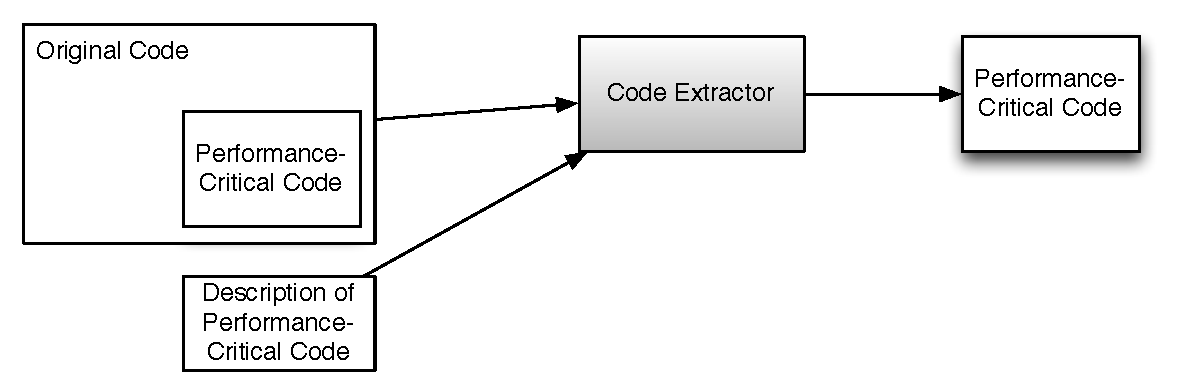
\includegraphics[width=\textwidth]{extractor.pdf}
\caption[Diagram of a code extractor]{Diagram of a code extractor, which isolates a section of code from its context, pulling it into its own scope so that it can be easily replaced with alternate implementations.}
\label{fig:extractor}
\end{figure}

\item[A method of adapting software to differing environments.]

Once the performance-critical routines have been isolated, we need a mechanism to create alternate versions which might have better performance. Creating alternate versions can be as simple as compiling the same code into multiple object files using different compilers, different levels of optimization, and/or different compiler flags. In this case, we will be primarily concerned with creating alternate versions by modifying input source code to create optimized output code, which can perform optimizations the compiler is not capable of making or exposes opportunities for optimizations the compiler is capable of making, but could not identify in the unmodified code. 

We will refer to a program capable of creating alternate versions of extracted code as a \textbf{code variant generator}. It takes source code as input, along with a description of possible code transformations which are optionally parameterized. For example, a transformation description could indicate that a loop should be unrolled; this can be parameterized by the number of times unrolling is to be applied. The function of a variant generator is depicted diagrammatically in Figure \ref{fig:variant}. Examples of variant generators include Orio \cite{orio,orio2,orio3}, POET \cite{poet} and CHiLL \cite{chill,full,rudy,interface,shreyas}.

\begin{figure}[tbp]
\centering
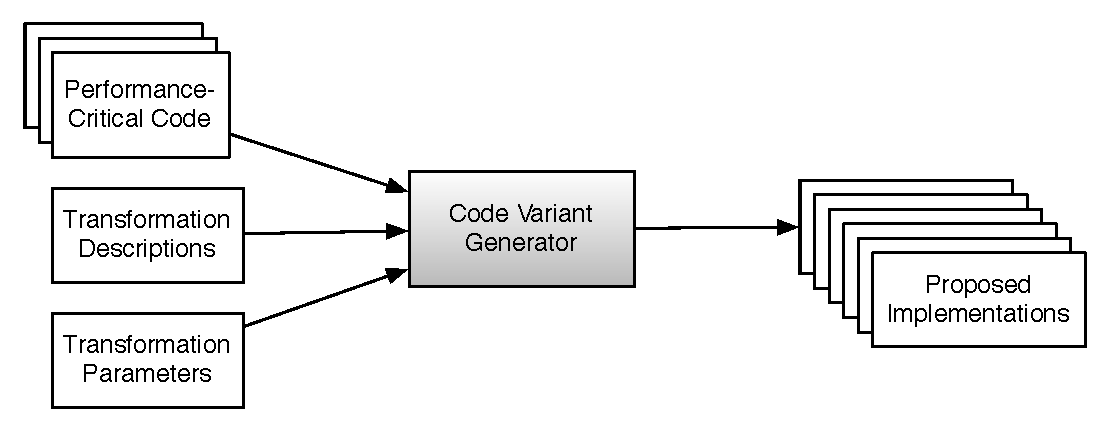
\includegraphics[width=\textwidth]{variant.pdf}
\caption[Diagram of a code variant generator]{Diagram of a code variant generator, which applies transformations to input code to generate a set of functionally-equivalent but differentially-performing output implementations.}
\label{fig:variant}
\end{figure}

\item[Robust, context-sensitive timers.]

Having generated a set of proposed code variants, we must execute them and measure their performance. In particular, we should measure their performance in such a manner that we do not severely perturb performance by our act of measurement.

We will refer to a program capable of timing code variants as a \textbf{performance measurement system}. It takes code variants as input and runs them with a set of representative input data, producing performance data tagged such that performance data can be associated with the implementation whose measurement generated the data. The function of a performance measurement system is depicted diagrammatically in Figure \ref{fig:performance}. Examples of performance measurement systems include HPCToolkit \cite{hpctoolkit} and TAU \cite{tau}.

\begin{figure}[tbp]
\centering
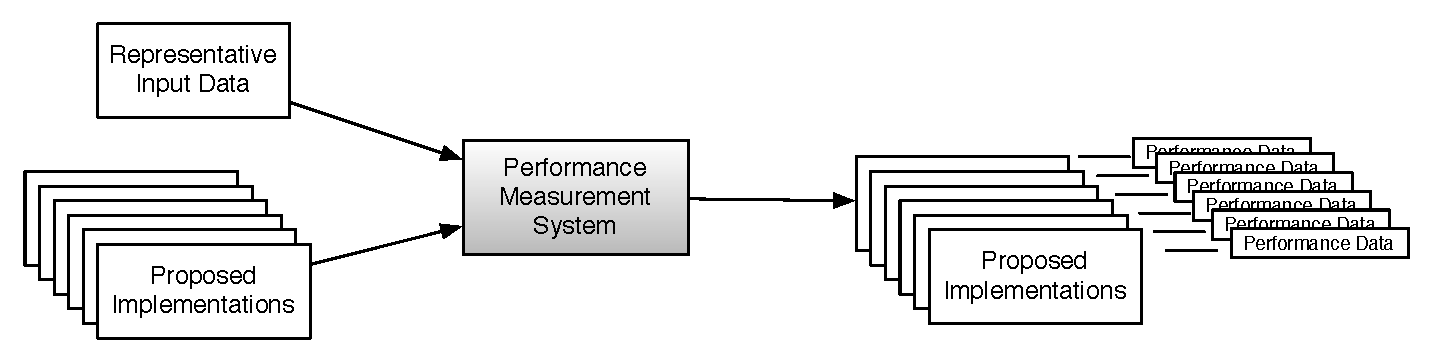
\includegraphics[width=\textwidth]{performance.pdf}
\caption[Diagram of a performance measurement system]{Diagram of a performance measurement system, which measures performance properties of code variants, producing data which are tagged such that performance data can be associated with variants.}
\label{fig:performance}
\end{figure}

\item[Appropriate search heuristics.]

It is often not feasible to exhaustively search the entire space of input parameters to the code variant generator, so some means of limiting the search space while still producing good results is needed. This is especially important if search is to be performed at runtime.

We will refer to a program capable of directing the search process as a \textbf{search engine}. It interfaces with the code variant generator and performance measurement system, selecting parameters to the code variant generator and then making a decision as to the next set of parameters to check based upon the performance characteristics of previously-tested variants. The function of the search engine within the context of the whole autotuning system is depicted diagrammatically in Figure \ref{fig:whole-system}. Examples of search engines include Active Harmony \cite{harmony,full,end-to-end,adaptive} and Orio \cite{orio,orio2,orio3}, the latter of which integrates a search engine and code variant generator into a single software package.

\begin{figure}[tbp]
\centering
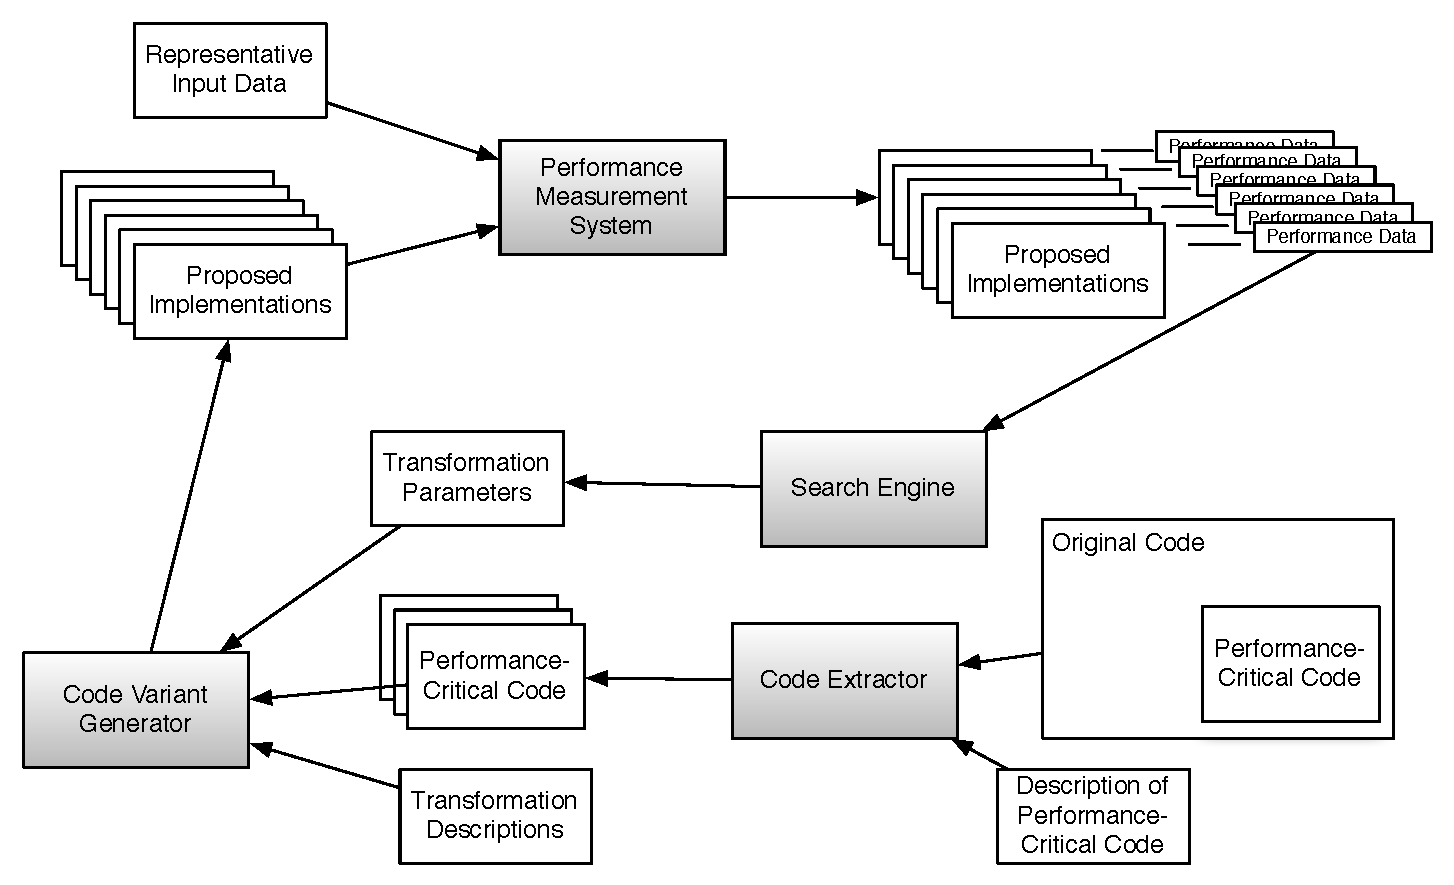
\includegraphics[width=\textwidth]{whole-system.pdf}
\caption[Diagram of a search-driven autotuning system]{Diagram of a search-driven autotuning system, in which a search engine selects parameters for the code variant generator based on past performance measurements.}
\label{fig:whole-system}
\end{figure}

\end{description}

\section{The ROSE/CHiLL/Active Harmony Stack}
\label{rosechill}

One general-purpose autotuning framework is proposed in \cite{full} and uses the ROSE outliner \cite{outlining} as the code isolator, CHiLL \cite{chill} as the code variant generator and Active Harmony \cite{harmony} as the search engine. This framework does not specify a particular performance measurement system; uses of this system in the past have used HPCToolkit \cite{hpctoolkit} or have involved calls to the PAPI \cite{papi} interface to directly access hardware performance counters. 

\subsection{The ROSE Outliner}

The ROSE outliner \cite{outlining} is based on the ROSE compiler system \cite{rose}, a compiler framework designed for source-to-source transformation. ROSE parses C, C++ and FORTRAN code into a common AST (abstract syntax tree) representation which can be traversed, analyzed, and modified. The modified AST can then be ``unparsed'' by ROSE, yielding a new source file which can be used as input to other tools.

The ROSE outliner allows the user to specify a section of code to be extracted into a separate function either using compiler pragmas or by ``abstract handles'' which allow position-independent references to nodes in the AST. During outlining, side-effect and liveness analyses are performed to determine whether it is possible to pass variables by value rather than by reference. By avoiding repeated pointer dereferences inside the outlined function wherever possible, the performance characteristics of the original block of code are maintained. Outlined kernels can be extracted to a separate source file which can then be used as input to a code variant generator.

\subsection{CHiLL}

CHiLL \cite{chill} is a code variant generator which allows the user to specify a series of high-level loop transformations to be applied together. CHiLL uses ROSE internally to parse code and applies transformations by making modifications to the ROSE AST. It uses a polyhedral model of loop transformations, in which the order of operations within nested loops are viewed as points inside a polyhedron, from which semantically-equivalent loops evaluating nests in different orders can be generated by applying geometric transformations to the polyhedron \cite{polytope}.

CHiLL recipes can be parameterized, and autotuning can be performed by searching the space of parameters to available recipes. An example of a CHiLL recipe with parameters is shown in Figure \ref{fig:chill-script}. In that recipe, three instances of loop tiling and two instances of loop unrolling are specified, but the parameters are left to be determined at a later point. For example, the variable \texttt{Ui} indicates the number of times loop 4 is to be unrolled. Table \ref{tab:chill-commands} lists some transformations CHiLL is capable of carrying out.

\begin{figure}[tbp]
\centering
\begin{verbatim}
permute([1,2,3])
tile(0,2,Tj)
tile(0,2,Ti)
tile(0,5,Tk)
unroll (0,4,Ui)
unroll (0,5,Uj)
\end{verbatim}
\caption{An example of a parameterized CHiLL recipe}
\label{fig:chill-script}
\end{figure}

\begin{table}[tbp]
\begin{center}
\begin{tabular}{ l | l }
\hline
Command & Meaning \\
\hline
\texttt{permute} & Change order of nested loops. \\
\texttt{tile} & Apply loop tiling to change order of loop iterations. \\
\texttt{split} & Split a loop with multiple statements in its body into multiple loops. \\
\texttt{fuse} & Inverse of split; combine multiple loops with the same loop boundaries into one loop. \\
\texttt{unroll} & Unroll loop (duplicate loop body and adjust loop boundaries) a specified number of times \\
\texttt{datacopy} & Copy data accessed by the loop into a contiguous block of memory \\
\hline
\end{tabular}
\end{center}
\caption{CHiLL recipe commands}
\label{tab:chill-commands}
\end{table}

CHiLL recipes also allow for known loop bounds to be expressed. This can enable optimizations which otherwise would not be available and is important for specialization. For example, if it is known that when the function being optimized is called with particular arguments that a loop will be executed a known number of times, a specialized variant could be generated in which the loop is fully unrolled.

A related tool is CUDA-CHiLL \cite{rudy}, which extends CHiLL with the ability to generate CUDA kernels for execution on GPUs from standard C or FORTRAN code. It adds a \texttt{cudaize} command which generates a CUDA kernel as well as commands for moving data around the CUDA memory hierarchy.

\subsection{Active Harmony}

Active Harmony \cite{harmony} is a search engine capable of rapidly exploring the parameter search space by testing multiple hypotheses in parallel, using the Parallel Rank Ordering algorithm to evaluate potential parameters. The user can specify parameters, ranges for the parameters, and constraints restricting the values parameters can take on. Active Harmony runs using a client-server architecture, in which a centralized Harmony server communicates with, and provides parameters to, multiple clients running on different, identically-configured nodes of a cluster. Additional servers can be configured as code servers, which perform compilation of code variants and distribute compiled object files to the execution nodes.

The architecture of Active Harmony is depicted diagrammatically in Figure \ref{fig:harmony}. 

\begin{figure}[tbp]
\centering
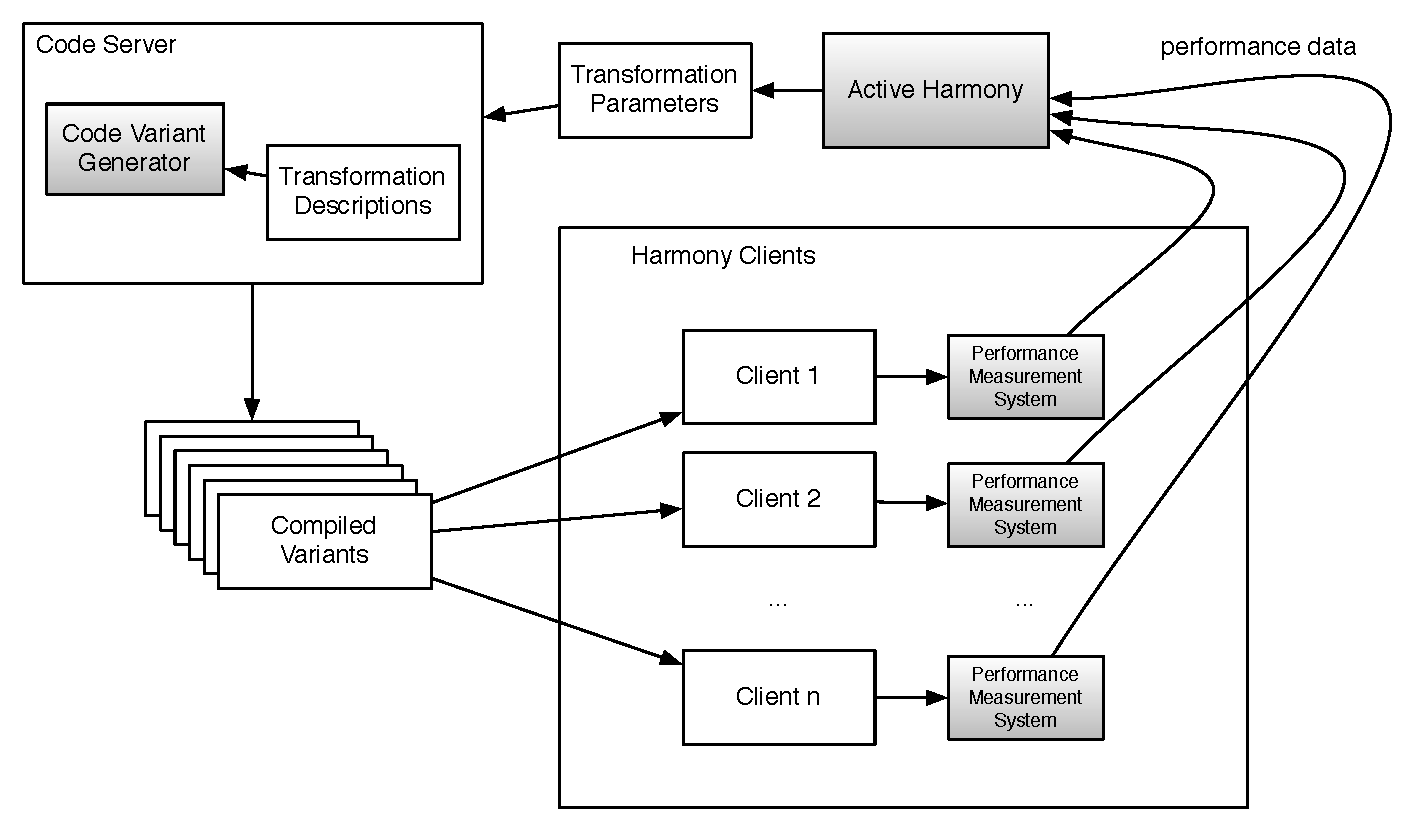
\includegraphics[width=\textwidth]{harmony.pdf}
\caption{Diagram of the Active Harmony architecture.}
\label{fig:harmony}
\end{figure}

\section{Case Studies}

Several papers have been published documenting the use of the ROSE/CHiLL/Active Harmony autotuning stack on production code.

\subsection{Dense Matrix Multiplication}
\label{dense}

In one case, autotuning and specialization were used to improve the performance of a dense matrix multiplication routine used by Nek5000, a fluid dynamics solver \cite{nek5000}. Shin et al. manually instrumented Nek5000 using PAPI calls to determine that 60\% of the total execution time was spent on a particular matrix multiplication routine, \texttt{mxm44\_0}. Having discovered this, \texttt{mxm44\_0} was manually instrumented by inserting code to capture the number of calls to the routine for each matrix size; this produced a histogram indicating the frequency with which different matrix sizes were encountered.

The frequency data showed that many multiplications over matrices of small sizes ($10 \times 10$ or smaller) were being performed, even though the BLAS libraries being used had been hand-tuned for large matrices: the routines were optimized to manage the cache hierarchy, but small matrices would fit into the L1 cache in their entirety. The researchers developed CHiLL recipes to unroll loops in the routine, using autotuning to identify the level of unrolling that would achieve peak performance (that is, the highest degree of unrolling that would not exhaust the instruction cache and/or supply of general purpose registers).

The researchers generated specialized versions of the matrix multiplication routine for the most frequently encountered matrix sizes, each having the empirically-determined ideal degree of unrolling for matrices of that size. They then wrote a script to generate a wrapper function which evaluates the size of input matrices and selects the optimal variant. The evaluation is done in order from most-frequent to least-frequent size encountered over the course of profiling, to minimize expected delay due to runtime variant selection. The use of these specialized variants improved performance by 2.2 times on a single node and 1.26 times when running in parallel on 256 nodes.

Note that the technique used in this study leaves room for further automation: performance instrumentation, parameter-gathering instrumentation, creation of specialized routines based on frequency of input parameters, and generation of an optimized wrapper function were either not automated or only partly automated. 

\subsection{Sparse Matrix Multiplication}
\label{sparse}

A study by Shreyas et al. \cite{shreyas} used CHiLL to create optimized, specialized variants of sparse matrix multiplication routines from the PETSc library. As in the Nek5000 study described above, the first step involved manually instrumenting the code to identify routines for optimization, then to instrument those routines specifically to capture parameter data. 

To optimize sparse matrix multiplication routines, alternate versions were written by hand which gathered data into a contiguous array of memory before the multiplication; both unmodified and gathering versions of the routines were subsequently put through the autotuning process. Recipes were written which performed loop unrolling, loop splitting and loop fusion to expose opportunities for the compiler to introduce vector instructions. Specialization was based upon a measure derived from the input data: the number of nonzero elements per row in the matrices.

This particular study did not require the use of Active Harmony or any other search engine, as the parameter spaces were sufficiently small that an exhaustive search could be performed in a reasonable amount of time. Using the optimized, specialized sparse matrix multiplication routines in three applications (PFLOTRAN, Uintah, and UNIC) yielded speedups ranging from 1.08 times to 1.87 times the original speeds.

\section{Limitations}

As exemplified by the studies described in Sections \ref{dense} and \ref{sparse} above, autotuning and specialization have great promise for improving the performance of software, but the process of using existing autotuning and specialization libraries is not sufficiently automated for their use to become mainstream. We would like some way for users to generate specialized function variants without the need for manual instrumentation, manual selection of parameters over which to specialize, and manual generation of replacement wrapper functions.

Therefore, in the next chapter, we will examine some uses of machine learning in selecting optimizations and discuss whether machine learning could be useful in selecting variants for specialization.
 
%%%%%%%%%%%%%%%%%%%%%%%%%%%%%%%%%%%%%%%%%%%%%%%%
%% CHAPTER THREE %%%%%%%%%%%%%%%%%%%%%%%%%%%%%%%
%% Machine Learning in Compiler Optimization  %%

\chapter{Machine Learning in Compiler Optimization}
\label{learning}

\section{Predicting Beneficial Optimizations}
\label{predicting}

One approach to the problem of selecting a specialized code variant is to train a classifier that maps from properties of the machine, code, or input data to a variant.

One of the earliest uses of this approach was that of Monsifrot et al. \cite{heuristics}, who studied the use of decision trees in selecting optimal unroll factors for loops extracted from the SPEC benchmarks. Their approach was to perform static analysis of the code to extract various descriptors of the code: number of statements, number of operations, number of array accesses, etc. Properties of the machine and input data were not considered. For each loop, the space of possible unroll factors was enumerated exhaustively and the performance of each was measured. By using decision tree learning over that dataset, a tree was produced which could, given a loop from the overall dataset omitted from the training dataset, identify the empirically-determined optimal unroll factor in 85.2\% of cases tested.

Stephenson and Amarasinghe \cite{unroll} used a similar approach --- static properties of the code to predict unroll factors --- with a larger number of code properties and with two different machine learning techniques: nearest-neighbor classification and support vector machines. 

Nearest-neighbor classifiers are very simple: using a distance measure defined over the features, the distance from the feature vector to be classified to existing feature vectors in the dataset is calculated and the new feature vector is assumed to map to the same classification as the nearest existing feature vectors. It has the advantage of being extremely fast to train and fast at classification. Nearest-neighbor classification was able to predict the optimal unroll factor on 62\% of test inputs.

Support vector machines are considerably more complicated classifiers; briefly, they transform the input data into a higher-dimensional space and find hyperplanes in that space which separate categories. For more details, see \cite{svm}. SVM classifiers trained on the same data as the nearest-neighbor classifiers were able to predict the optimal unroll factor on79\% of test inputs, but require more time to carry out the training algorithm. They have the additional limitation of being difficult to interpret by humans; general rules cannot be easily inferred by inspecting a support vector machine.

While the two studies discusses above used static code properties as input, a study by Cavazos et al. \cite{counters} uses performance counter data collected at runtime, and is therefore more directly applicable to the problem of autotuning. Their approach involves first testing a large number (around 500) of randomly selected combinations of compiler optimization flags and recording execution time along with the values stored in various hardware counters (e.g., numbers of adds, multiplies, subtractions, divisions; number of branches taken, not taken, mispredicted; data and instruction cache hits and misses; etc.). Logistic regression is then used to assign to each compiler optimization a probability indicating whether it should be evaluated given the performance counter data. Future autotuning is then driven by selecting and evaluating optimizations based upon the probabilities determined from the logistic regression model. This method was highly successful, improving the performance of the SPEC benchmarks by 17\%. However, this method does not take static properties of the code or the input dataset into consideration except indirectly though their effects on performance counters.

Other approaches for using machine learning to generate optimized code variants include generating algorithms by composing blocks of code together; for example, this technique has been used with genetic algorithms to produce specialized sorting algorithms \cite{sorting} and with XCS classifier learning systems to produce specialized matrix multiplication algorithms \cite{classifier}.

\section{Collective Tuning}

A very interesting approach is taken by Fursin and Temam \cite{collective}, which they name \emph{collective optimization}. Their approach differs from the standard autotuning approach described in Chapter \ref{autotuning} and from the machine learning techniques described in Section \ref{predicting} in that it does not explicitly search a parameter space, but rather adjusts a centrally-maintained set of probability distributions in response to input data submitted from clients running instrumented applications across platforms and datasets. 

The collective tuning approach uses a modified version of GCC which implements function cloning. When a source file is compiled, functions of interest are cloned, one of which is left in its original state, and the other of which is optimized according to an optimization selected by an approach similar to that used by Cavazos et al. \cite{counters} as described in Section \ref{predicting}. It is initially not known whether the original or the optimized code variant will provide better performance on the dataset about to be used, so a uniform distribution is used at runtime to select a variant to use each time the original function is called --- that is, there is initially a 50\% chance that the original version will be called, and a 50\% chance that the optimized version will be called upon each invocation of the function. 

Since the probability of each function being called is known, the proportion of time spent in each function should match those probabilities assuming the the functions have equal performance. If the proportion of time spent in a function is significantly lower than the expectation assuming equality, then it can be inferred that that variant offers better performance than its competitor. The result of the competition is then communicated to a central server which updates probability distributions: one probability distribution for the program, another which aggregates data for programs with similar reactions to optimizations, and a third which aggregates data across all programs.

In this way, the collective tuning approach is able to adjust to data learned over time across environments and datasets. It shows the importance of being able to aggregate performance data from many sources in order to get the most benefit from machine learning techniques.

\section{Decision Tree Learning}
\label{tree}

A \emph{decision tree} is a DAG (directed acyclic graph) in which interior nodes represent ``decisions'', fields in which the input feature vectors differ; the leaf nodes represent classifications and edges represent particular values which can be taken on by the field represented by the node from which the edge emanates. In autotuning, our feature vectors include data about the programs being executed, the environment in which the programs are being executed, and the input data to the programs. Classifications are code variants or instructions for generating code variants (e.g., a parameterized recipe and its parameters). An example of such a decision tree is shown in Figure \ref{fig:dectree}.

\begin{figure}[tbp]
\centering
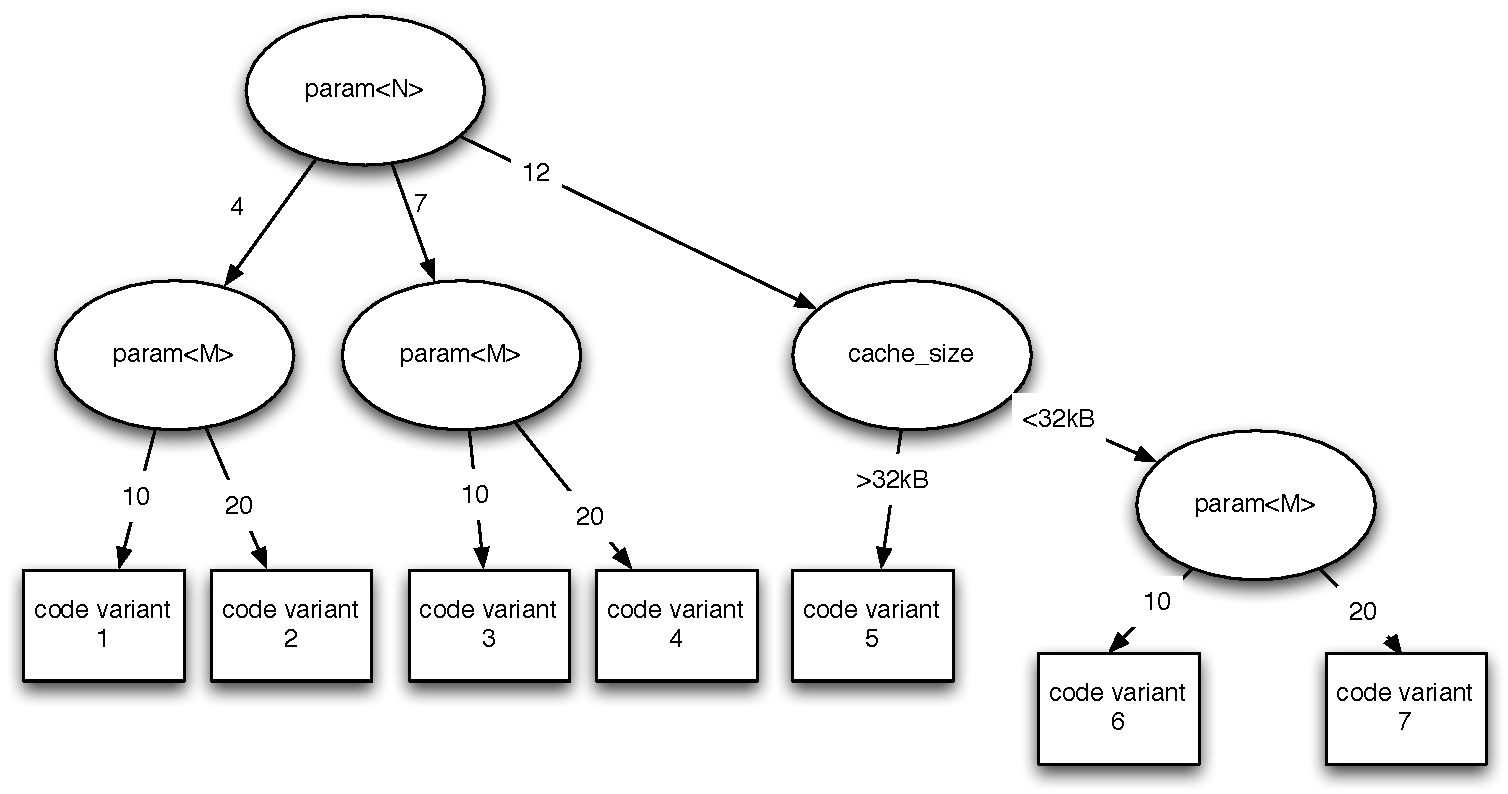
\includegraphics[width=\textwidth]{dectree.pdf}
\caption{A decision tree for selecting code variants from input data and execution environment data.}
\label{fig:dectree}
\end{figure}

The most common decision tree learning algorithms are ID3 \cite{id3} and C4.5 \cite{c45}, both due to Ross Quinlan. These learn short trees in which the most informative nodes tend to be located closer to the root. Both algorithms select nodes greedily, picking the node which currently gives the highest information gain, defined as $$Gain(S,A) \equiv Entropy(S) - \sum\limits_{v \in Values(A)} {{\left|S_v\right|}\over{S}}\ Entropy(S_v)$$ where $$Entropy(S) \equiv \sum\limits_{i=1}^c -p_i\log_2 p_i\mathrm{.}$$

ID3 uses information gain directly, while C4.5 adds the ability to substitute a leaf node for an interior node if the loss in information is sufficiently small, thereby reducing the amount of time needed for classification. Reducing the time needed for classification is useful if we are using these trees to select optimized code variants, as we could potentially offset the improved performance in using specialized variants if we take too much time picking which variant to use. The Weka machine learning library \cite{weka} provides a customized variant of C4.5 called J48 which we will use in Chapter \ref{design} in the development of a system for autotuning and specialization.


%%%%%%%%%%%%%%%%%%%%%%%%%%%%%%%%%%%
%% CHAPTER FOUR %%%%%%%%%%%%%%%%%%%
%% Design and Implementation %%%%%%

\chapter{Design and Implementation of an Autotuning Framework}
\label{design}

\section{Goals}
\label{goals}

Let us reiterate our goals in developing an autotuning framework:

\begin{itemize}
\item Automatically gather metadata describing \textbf{properties of the input data} to the program being tuned, so that we can later specialize based on those properties.
\item Automatically gather metadata describing \textbf{the execution environment} of the program being tuned, so that we can later specialize based on those properties.
\item Automatically \textbf{learn a decision tree classifier} which maps the gathered properties of the input data and execution environment to a choice of code variant.
\item Automatically generate \textbf{executable code from the decision tree} to perform the classification at runtime.
\end{itemize}

We will use the ROSE/CHiLL/Active Harmony stack described in Section \ref{rosechill}, augment it with parameterized profiling, metadata capture into a performance database, decision tree learning and wrapper function generation and develop a driver program to automatically configure ROSE, CHiLL and Active Harmony to work together with these augmentations.

\section{Parameterized Profiling with TAU}
\label{param}

We extended TAU \cite{tau}, a performance measurement system, to support gathering parameters to functions. For example, if we are autotuning and specializing a matrix multiplication routine, TAU can be configured to gather data on the frequency with which each size matrix was encountered, as well as separate performance statistics for the routine when called on differently-sized matrices. An example of this is shown in Table \ref{tab:parameterized}

TAU automatically instruments C, C++ and FORTRAN source files, inserting calls to timer routines at the start and end of functions, and, optionally, loops, taking advantage of PDT (Program Database Toolkit) files \cite{pdt}, which describe, among other properties, functions and their arguments. Using this information routines can also be inserted at the start and end of functions to run timer routines specific to the arguments with which the function was called. 

Because PDT does not capture data about local variables, and it is often useful to parameterize based upon a derived property of the actual function arguments stored in a local variable, we also developed a ROSE-based tool which inserts parameterized timer code based upon a ROSE abstract handle.

Initial performance measurements are stored in a performance database, namely PerfDMF (or TauDB, a newer version of the same software), which will be described in more detail in section \ref{perfdmf}.

To add parameterized profiling to the autotuning framework, it is inserted as a new phase after code extraction, as shown in Figure \ref{fig:instrument}

\begin{figure}[tbp]
\centering
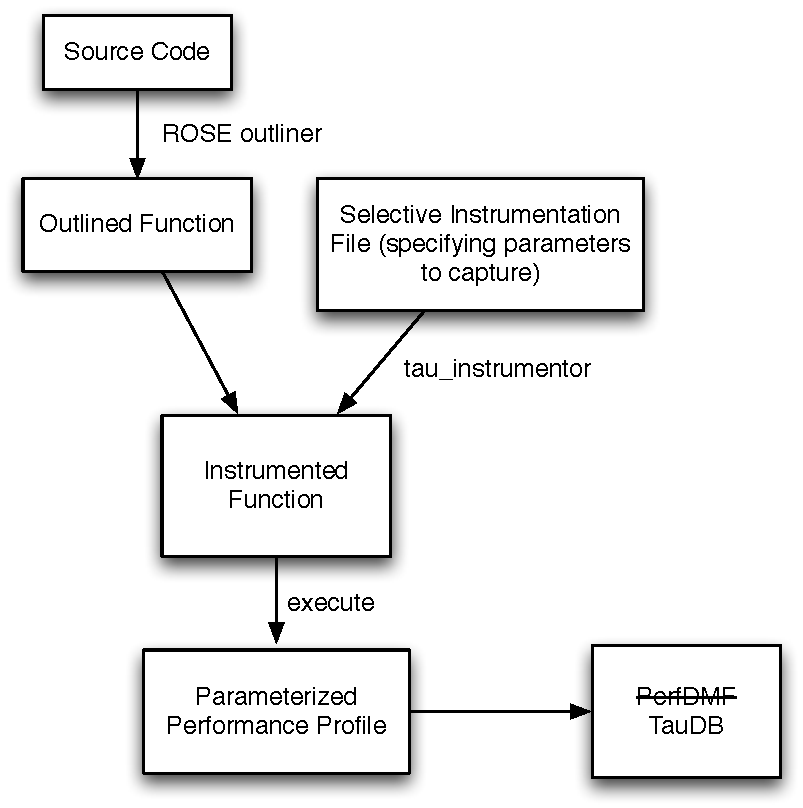
\includegraphics[width=0.5\textwidth]{instrument.pdf}
\caption{Diagram of a portion of the autotuning workflow, showing parameterized profiling.}
\label{fig:instrument}
\end{figure}

\begin{table}[tbp]
\begin{center}
\begin{tabular}{ r | r | r | l }
\hline
\% & msec & Calls &  Name \\
\hline
6.2&2,753&100&void matMult(size\_t, float *, float *, float *) [ <size> = <256> ] \\
0.7&  307&100&void matMult(size\_t, float *, float *, float *) [ <size> = <128> ] \\
0.1&   38&100&void matMult(size\_t, float *, float *, float *) [ <size> = <64> ] \\
0.0&    7&100&void matMult(size\_t, float *, float *, float *) [ <size> = <32> ] \\
0.0&    1&100&void matMult(size\_t, float *, float *, float *) [ <size> = <16> ] \\
0.0&    1&100&void matMult(size\_t, float *, float *, float *) [ <size> = <2> ] \\
0.0&0.991&100&void matMult(size\_t, float *, float *, float *) [ <size> = <8> ] \\
0.0&0.885&100&void matMult(size\_t, float *, float *, float *) [ <size> = <4> ] \\
\hline
\end{tabular}
\end{center}
\caption{Performance data parameterized by input metadata}
\label{tab:parameterized}
\end{table}

\section{Capturing Metadata in PerfDMF}
\label{perfdmf}

PerfDMF \cite{perfdmf} is a performance measurement database designed to store performance measurements of sequential and parallel applications over the course of multiple experiments. It provides for multiple clients to submit performance data to a central repository, where it can be analyzed in aggregate. Usefully for our current task, it also features robust support for the storage of metadata --- both standard metadata automatically gathered by TAU as well as user-specified metadata.

By virtue of using TAU to gather performance data and storing those data in PerfDMF, we automatically capture a large amount of information about the execution environment. Table \ref{tab:metadata} shows default metadata about the execution environment that the framework captures on all systems. When we use parameterized profiling, as described in Section \ref{param}, parameters are stored as part of the names of timers and are therefore also accessible. A new version of PerfDMF currently under development, called TauDB, will provide additional support for parameterized profiles, allowing, for example, efficient range-based queries over function parameters. 

We also capture metadata pertaining to the input data, namely, parameters to instrumented functions, as well as \emph{provenance} data, indicating where the code being tested came from: is it the original, unoptimized code; a hand-tuned variant; or was it produced by a code variant generator, and, if so, which code variant generator, using which script and which parameters? Table \ref{tab:userdata} shows default metadata about input data and provenance.

Performance measurements are stored in PerfDMF for both the initial runs to gather parameter data, and for each CHiLL variant tested during the autotuning process, as driven by Active Harmony. We developed an Active Harmony driver which interfaces with PerfDMF to store intermediate results in the database and use TAU metrics as the value to be optimized by the search process. The driver instruments each CHiLL-produced variant using PDT and TAU. The overall workflow of this stage is depicted diagrammatically in Figure \ref{fig:autotune}.

\begin{table}[btp]
\begin{center}
\begin{tabular}{ l | l}
\hline
Metadata Type \\
\hline
Execution start time \\
Hostname & Process ID (pid) \\
OS Name & CPU Vendor \\
OS Version & CPU Clock Speed \\
OS Release & CPU Type \\
TAU Architecture & CPU Cache Size\\
TAU Configuration & CPU Number of Cores\\
TAU Makefile & Host Memory Size\\
TAU Version & Executable Name\\
Current working directory & Command line arguments \\
Compiler name used & Compiler version \\
\hline
\end{tabular}
\end{center}
\caption{Execution environment metadata captured by default}
\label{tab:metadata}
\end{table}

\begin{table}[btp]
\begin{center}
\begin{tabular}{ l }
\hline
Metadata Type \\
\hline
Parameters to instrumented functions \\
Name of transformation recipe used, if any \\
Values of transformation parameters, if any \\
Transformation system used (e.g., CHiLL), if any \\
Transformation system version, if any \\
\hline
\end{tabular}
\end{center}
\caption{Other metadata captured by default}
\label{tab:userdata}
\end{table}

\begin{figure}[tbp]
\centering
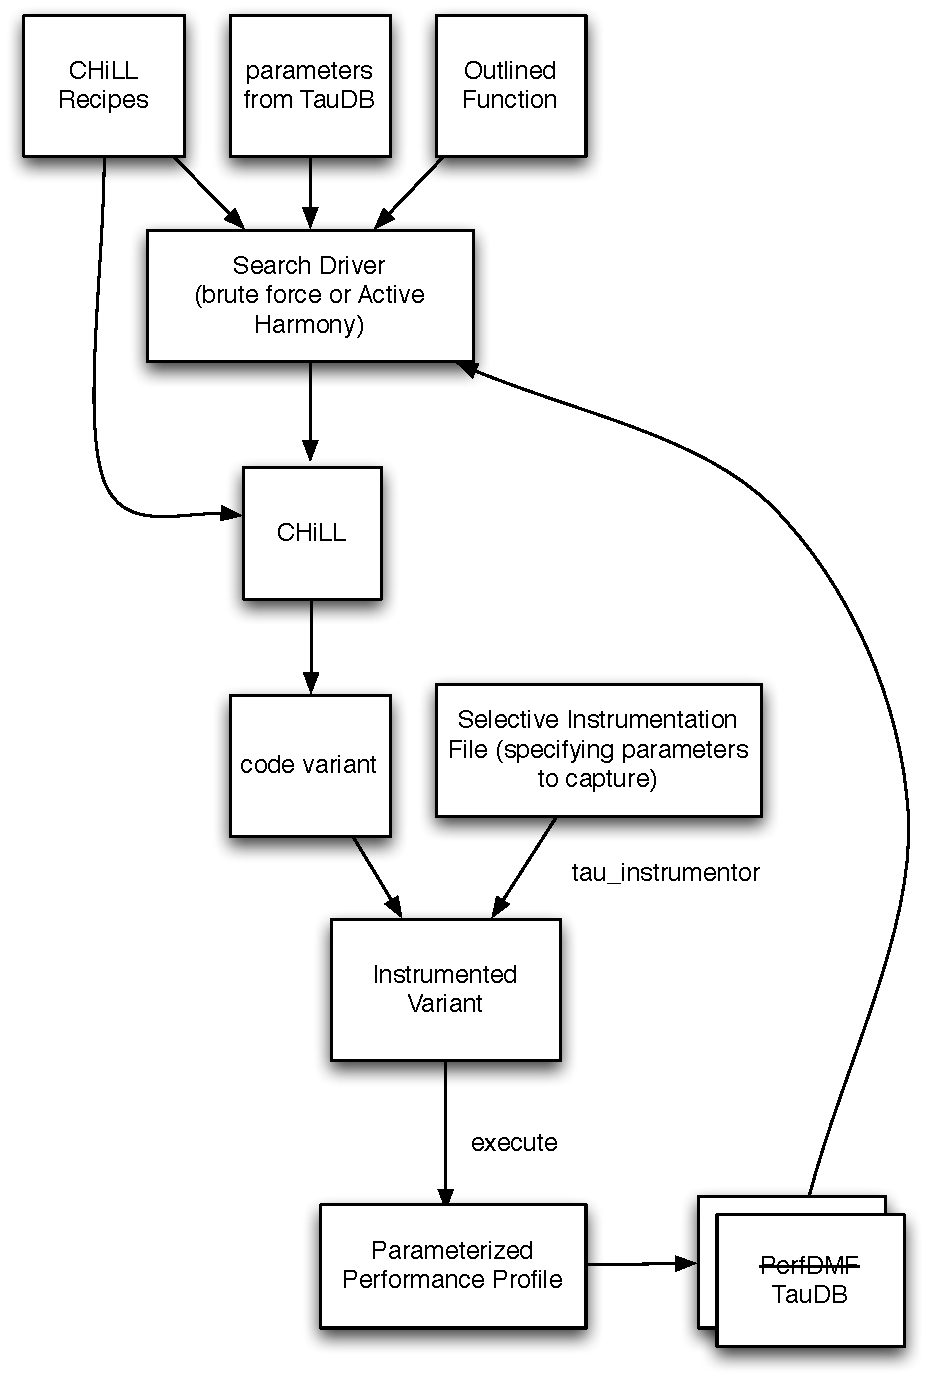
\includegraphics[width=0.80\textwidth]{autotune.pdf}
\caption[Diagram of data being stored in PerfDMF]{Diagram of a portion of the autotuning workflow, showing performance data during search being stored in the PerfDMF performance database.}
\label{fig:autotune}
\end{figure}

\section{Decision Tree Learning with PerfDMF and Weka}
\label{treelearn}

Now that performance data annotated with environmental and input-data-based metadata are stored in a PerfDMF database, we can learn a decision tree taking the described set of metadata as the feature vector and the provenance metadata as the label. We use the J48 algorithm provided by Weka \cite{weka}, a Java-based machine learning library. J48 is appropriate because it supports pruning uninformative nodes from decision trees as well as range-based decisions (e.g., an edge for cache size between 1 and 2 MB). Weka was used because it is already in use inside the TAU project as part of PerfExplorer \cite{perfexplorer}, a program for performing data mining on parallel performance data.

Once a decision tree has been generated, it is read by a ROSE-based tool which constructs the AST of a wrapper function and unparses it to C or C++ code. The wrapper function is then inserted into the original source code in place of the function which has been specialized. The wrapper function represents the tree as a series of if-then-else statements (for binary decision trees) or switch statements (for \emph{n}-ary decision trees where $n > 2$). J48 is biased towards short trees with the most informative nodes located near the root, meaning that the wrapper functions generated should tend to evaluate the most likely cases first and should not have to evaluate too many cases in order to determine which code variant to execute.

Code to evaluate each decision node is provided for each of the default types of metadata generated by the framework. This code takes the form of an inlineable function annotated with a compiler pragma indicating the name of the metadata node it decides. The wrapper generator will replace calls to the decision function with the function body in the wrapper function to avoid introducing overhead from function calls.

Not all data in the feature vector may be available on all systems. Therefore, clients can send a request to a decision tree server listing which metadata are actually available and which application is being run. The server will then generate a custom decision tree including only relevant nodes.

Figure \ref{fig:wrapgen} depicts diagrammatically the workflow of this stage of the framework.

\begin{figure}[btp]
\centering
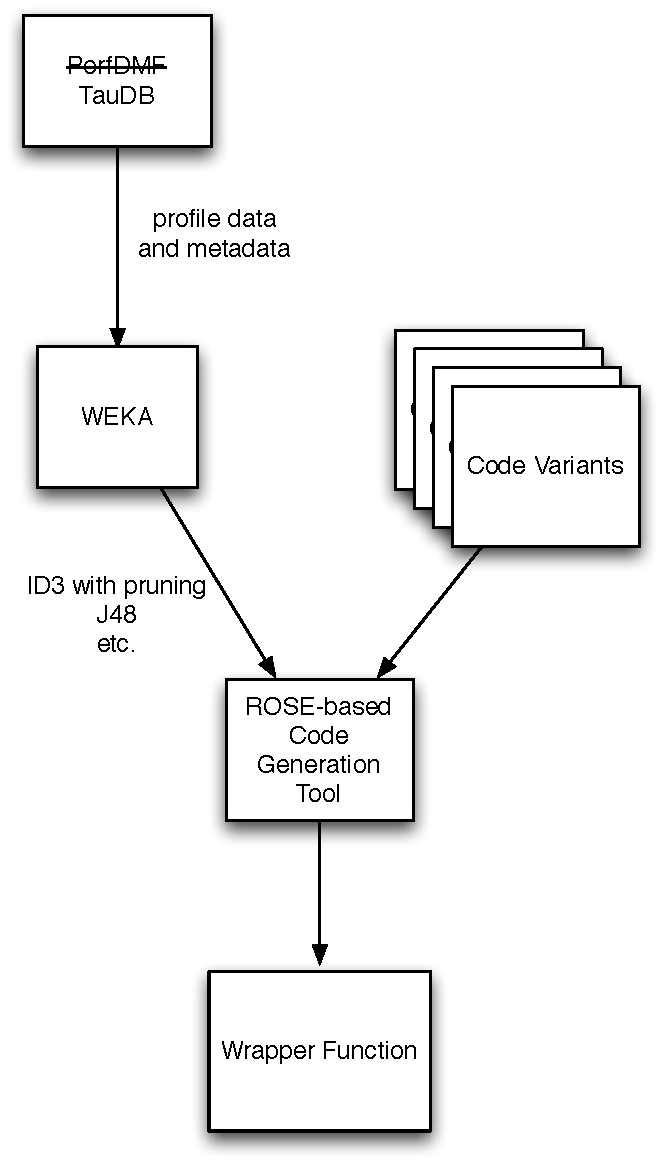
\includegraphics[width=0.50\textwidth]{wrapgen.pdf}
\caption[Diagram of decision tree learning and wrapper generation]{Diagram of a portion of the autotuning workflow, showing decision tree learning and wrapper generation.}
\label{fig:wrapgen}
\end{figure}

\section{Conclusion}
\label{architecture}

This chapter showed how we have implemented automated generation of specialized function variants in the ROSE/CHiLL/Active Harmony-based autotuning framework by integrating those tools with TAU, PerfDMF, Weka, and a custom-built wrapper generator. Chapter \ref{results} will show examples of this framework being used to generate such specialized functions.

%%%%%%%%%%%%%%%%%%%%%%%%%%%%%%%%%%%
%% CHAPTER FIVE %%%%%%%%%%%%%%%%%%%
%% EMPIRICAL EVALUATION %%%%%%%%%%%

\chapter{Empirical Evaluation}
\label{results}

This chapter shows how the autotuning and specialization framework described in Chapter \ref{design} can be applied to specializing based on input parameters, specializing based on architectural features, and specializing based on both input parameters and architectural features.

\section{Specializing Based on Input Data}
\label {inputdata}

\begin{figure}[btp]
\begin{subfigure}[b]{0.45\textwidth}
\centering
\scriptsize\begin{verbatim}
for(j=0; j < n; j++) {
  for(k=0; k < n; k++) {
    for(i=0; i < n; i++) {
        c[i][j] =c[i][j] + a[i][k]*b[k][j];
    }
  }
}
\end{verbatim}
\caption{Na\"{\i}ve implementation of \\ matrix multiply}
\label{fig:multiply}
\end{subfigure}\hspace{2pt}
\begin{subfigure}[b]{0.3\textwidth}
\centering
\scriptsize\begin{verbatim}
permute([3,1,2])
tile(0,2,TJ)
tile(0,2,TI)
tile(0,5,TK)
datacopy(0,3,a,false,1)
datacopy(0,4,b)
unroll(0,4,UI)
unroll(0,5,UJ)
\end{verbatim}
\caption{\centering CHiLL recipe for large matrices}
\label{fig:large}
\end{subfigure}\hspace{2pt}
\begin{subfigure}[b]{0.2\textwidth}
\centering
\scriptsize\begin{verbatim}
permute([1,2,3])
unroll(1,1,U1)
unroll(1,2,U2)
unroll(1,3,U3)
\end{verbatim}
\caption{\centering CHiLL recipe for small matrices}
\label{fig:small}
\end{subfigure}
\caption{Matrix multiplication and sample transformation recipes}
\label{fig:inputdatat}
\end{figure}

This experiment analyzed the optimization of a basic matrix multiply routine shown in Figure \ref{fig:multiply}. As noted in describing the specialization of the matrix multiplication in Nek5000 \cite{nek5000} in Section \ref{dense}, optimization of matrix multiply for large matrices involves performing loop tiling to manage the memory hierarchy, whereas optimization of matrix multiply for small matrices does not require loop tiling, and consists primarily of loop unrolling. 

Therefore, the autotuning framework was configured to use CHiLL recipes which perform loop tiling and loop unrolling, expected to improve performance on large matrices, and CHiLL recipes which perform loop unrolling but not loop tiling, expected to improve performance on small matrices. Examples of these recipes are shown in Figures \ref{fig:large} and \ref{fig:small}. Other recipes used are similar but perform different permutations of the loop nests. An example of a generated code variant is shown in Figure \ref{fig:codevariant}.

A driver program was written which repeatedly calls the matrix multiply routine on square matrices of differing sizes. The autotuning framework was configured to instrument the matrix multiply routine to parameterize performance data based on matrix size. Autotuning was performed on the ACISS cluster at the University of Oregon using CHiLL and Active Harmony, and with performance measurements being saved into PerfDMF. Code variants were compiled with the Intel C compiler. Four final code variants were generated: the unchanged original version, the best variant found from among the tile-and-unroll tests, the best variant found from among the unroll-only tests, and the automatically generated wrapper based upon the learned decision tree (which split between the two generated variants at size $N = 1024$). 

\begin{figure}[tbp]
\centering
\scriptsize\begin{verbatim}
  for (t2 = 0; t2 <= n - 1; t2 += 512) {
    for (t4 = 0; t4 <= n - 1; t4 += 128) {
      for (t6 = t4; t6 <= __rose_lt(n - 1,t4 + 127); t6 += 1) {
        for (t8 = t2; t8 <= __rose_lt(t2 + 511,n - 1); t8 += 1) {
          _P1[t6 - t4][t8 - t2] = a[t6][t8];
        }
      }
      for (t6 = 0; t6 <= n - 1; t6 += 8) {
        for (t8 = t2; t8 <= __rose_lt(n - 1,t2 + 511); t8 += 1) {
          for (t10 = t6; t10 <= __rose_lt(n - 1,t6 + 7); t10 += 1) {
            _P2[t8 - t2][t10 - t6] = b[t8][t10];
          }
        }
        over1 = n % 2;
        for (t8 = t4; t8 <= __rose_lt(-over1 + n - 1,t4 + 126); t8 += 2) {
          over2 = n % 2;
          for (t10 = t6; t10 <= __rose_lt(n - over2 - 1,t6 + 6); t10 += 2) {
            for (t12 = t2; t12 <= __rose_lt(t2 + 511,n - 1); t12 += 1) {
              (c[t8])[t10] = (((c[t8])[t10]) + (_P1[t8 - t4][t12 - t2] * _P2[t12 - t2][t10 - t6]));
              (c[t8 + 1])[t10] = (((c[t8 + 1])[t10]) + (_P1[t8 + 1 - t4][t12 - t2] * _P2[t12 - t2][t10 - t6]));
              (c[t8])[t10 + 1] = (((c[t8])[t10 + 1]) + (_P1[t8 - t4][t12 - t2] * _P2[t12 - t2][t10 + 1 - t6]));
              (c[t8 + 1])[t10 + 1] = (((c[t8 + 1])[t10 + 1]) + (_P1[t8 + 1 - t4][t12 - t2] * _P2[t12 - t2][t10 + 1 - t6]));
            }
          }
          if (n <= t6 + 8 && 1 <= over2) 
            for (t12 = t2; t12 <= __rose_lt(n - 1,t2 + 511); t12 += 1) {
              (c[t8])[n - 1] = (((c[t8])[n - 1]) + (_P1[t8 - t4][t12 - t2] * _P2[t12 - t2][n - 1 - t6]));
              (c[t8 + 1])[n - 1] = (((c[t8 + 1])[n - 1]) + (_P1[t8 + 1 - t4][t12 - t2] * _P2[t12 - t2][n - 1 - t6]));
            }
        }
        if (1 <= over1 && n <= t4 + 128) 
          for (t10 = t6; t10 <= __rose_lt(t6 + 7,n - 1); t10 += 1) {
            for (t12 = t2; t12 <= __rose_lt(t2 + 511,n - 1); t12 += 1) {
              (c[n - 1])[t10] = (((c[n - 1])[t10]) + (_P1[n - 1 - t4][t12 - t2] * _P2[t12 - t2][t10 - t6]));
            }
          }
      }
    }
  }
\end{verbatim}
\caption{A variant generated for the matrix multiply kernel from the tile-and-unroll script}
\label{fig:codevariant}
\end{figure}

\begin{figure}[btp]
\centering
\scriptsize\begin{verbatim}
/* VALID: user_PARAM<n> */
void gemm_WRAP_g1_out(size_t n, double * a, double * b, double * c) {
  /* NODE: user_PARAM<n> LEFT: v106 RIGHT: v284 */
  if(n*n > 1024) {
    rose_gemm_VAR_t_v106i(n, a, b, c);
  } else {
    rose_gemm_VAR_l_v284i(n, a, b, c);
  }
}
\end{verbatim}
\caption[An auto-generated wrapper function]{A simple example of an auto-generated wrapper function.}
\label{fig:wrapperfun}
\end{figure}


The code variants were tested on three types of workloads: entirely small matrices ($n <= 32$), entirely large matrices ($n > 32$), or a mixed workload consisting of half large and half small matrices.  Results are shown in Figure \ref{fig:perf_chart}. The wrapped version achieved the best overall performance on a mixed workload, indicating that the autotuning system was successful in specializing for the cases present in the input data.

\begin{figure}[btp]
\centering
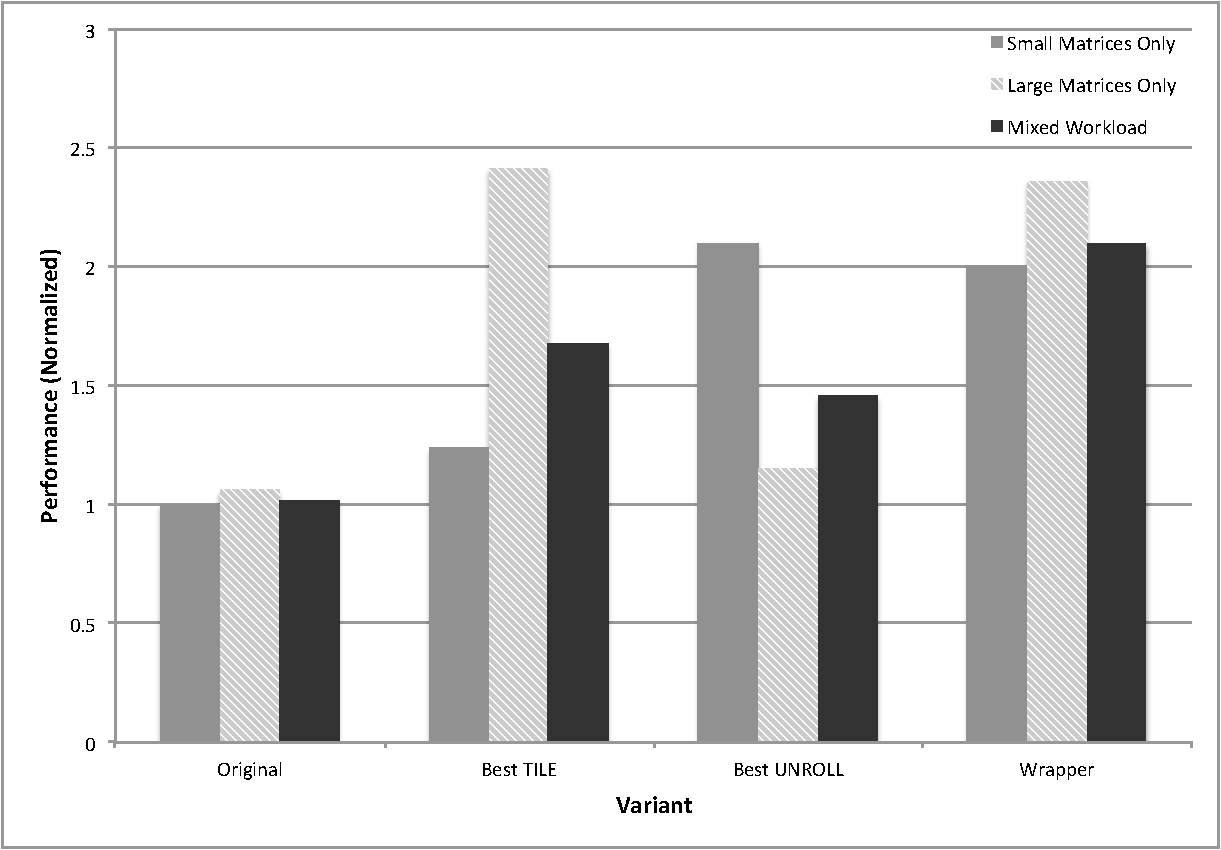
\includegraphics[width=\textwidth]{perf_chart.pdf}
\caption[Normalized performance of dense matrix multiply variants]{Normalized performance of dense matrix multiply variants on small, large or mixed workloads.}
\label{fig:perf_chart}
\end{figure}

\section{Specializing a CUDA Kernel Based on Execution Environment}
\label{cudakernel}

Another experiment was performed to determine whether the autotuning system could specialize based upon differences in hardware. For this experiment, CUDA matrix multiply kernels were generated using CUDA-CHiLL \cite{rudy} from the same initial code as in the experiment of Section \ref{inputdata}, but using a different CHiLL script, shown in Figure \ref{fig:cudascript}. The script was provided by Suchit Maindola of the University of Utah [personal communication]. Note that CUDA-CHiLL uses a different script syntax than standard CHiLL; whereas CHiLL uses a custom language, CUDA-CHiLL scripts are Lua scripts and allow references to loops by the name of their index variable, instead of merely by nest level.

\begin{figure}[btp]
\centering
\scriptsize\begin{verbatim}
init("cudamm.cu", "cudamm", 0) 
dofile("cudaize.lua")

N=1024
TI=@TI@
TJ=@TJ@
TK=@TK@

tile_by_index({"i","j"}, {TI,TJ}, {l1_control="ii", l2_control="jj"}, {"ii", "jj", "i", "j"})
tile_by_index({"k"}, {TK}, {l1_control="kk"}, {"ii", "jj", "kk","i", "j","k"}, strided)

tile_by_index({"i"}, {TJ}, {l1_control="tt",l1_tile="t"}, {"ii", "jj", "kk","t","tt","j","k"})

cudaize("cudamm_GPU", {a=N*N, b=N*N, c=N*N}, {block={"ii","jj"}, thread={"t","tt"}})
copy_to_shared("tx", "b", -16)

copy_to_registers("kk","c")
unroll_to_depth(2)
\end{verbatim}
\caption{CUDA-CHiLL script used to generate CUDA matrix multiply kernels.}
\label{fig:cudascript}
\end{figure}

Active Harmony was used to direct the search of the space of TI, TJ, and TK parameters to the CUDA-CHiLL script, which control the tile sizes used. CUDA-CHiLL generates CUDA kernels from the serial C code, and generates a wrapper function which invokes the CUDA kernel. An example of a matrix multiply kernel generated by CUDA-CHiLL is presented in Appendix A. TAUcuda \cite{taucuda} was used to profile the CUDA kernels over the CUDA CUPTI interface. Autotuning was performed on an NVIDIA S1070, an NVIDIA C2070, and an NVIDIA GTX 480. Data on which type of GPU was present on each system was stored as metadata in PerfDMF so that this could be used in decision tree generation.

The autotuning system found that the best-performing variant for the NVIDIA C2070 and GTX 480 was TI=64, TJ=16, TK=16, while the best-performing variant for the NVIDIA S1070 was TI=64, TJ=32, TK=32. The autotuning system is capable of generating specialized variants based upon differences in hardware between systems.

\section{Specializing Based on Input Data and Execution Environment in a Virtualized Environment}

Finally, an experiment was performed to determine whether the autotuning system can handle cases where a difference in performance is due to an interaction between properties of the input data and properties of the execution environment. This test was carried out in a virtualized environment to demonstrate the usefulness of the autotuning technique in the cloud, where an installation of the software installed on a virtual disk image may find itself running in different environments at different times.

For this experiment, CHiLL was not used. Rather, variants of a sorting function were specified manually: specifically, one variant loaded the data to be sorted into memory and used the standard C++ STL sort function, while the other used a disk-based external sort from STXXL \cite{stxxl}, a C++ library intended for use on data too large to fit into memory. A program was written to sort small (512 MB) or large (4 GB) files. Once this was set up, a disk image was saved and virtual machine instances were launched with either 2 GB or 8 GB of RAM. These instances communicated with a central Active Harmony server which in turn communicated with PerfDMF. 

The system was able to learn a decision tree --- and hence generate a wrapper function --- which selects the in-memory sort for small files regardless of whether the test occurred on a small-RAM or large-RAM instance; the decision tree is shown in Figure \ref{fig:vm_exp}. Note, however, that the decision tree shows a limitation of the learning algorithm: since only two file sizes were present in the test input, only two file sizes are present in the test output. If the classifier encounters a previously unknown filesize, it will receive a default classification, which is not what is desired. The wrapper function can be modified to use ranges, but this must be done manually. While the system recognizes that there is some relation between file size and the amount of RAM available to the instance, it does not learn that there is a direct causal relationship.

\begin{figure}[btp]
\centering
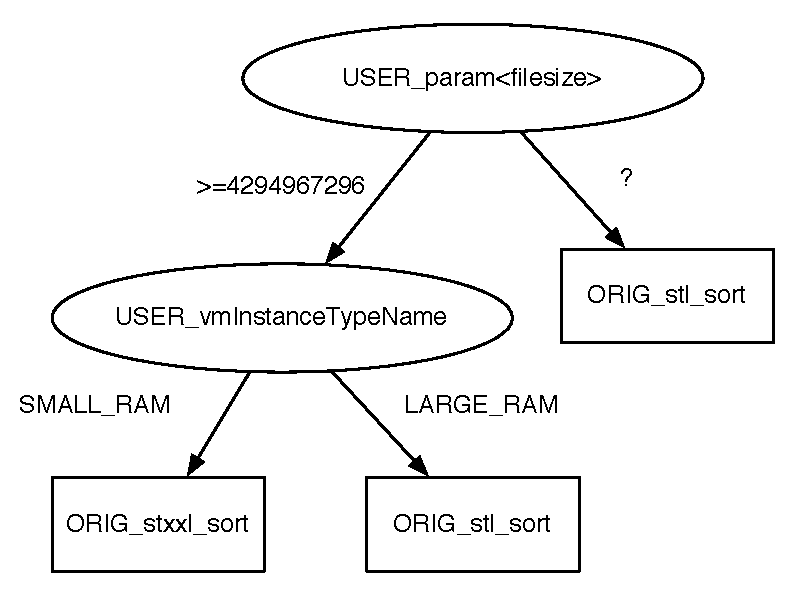
\includegraphics[width=0.8\textwidth]{vm_exp.pdf}
\caption{Decision tree learned for the virtualized environment experiment.}
\label{fig:vm_exp}
\end{figure}


%%%%%%%%%%%%%%%%%%%%%%%%%%%%%%%%%%%
%% CHAPTER SIX %%%%%%%%%%%%%%%%%%%%
%% CONCLUSION %%%%%%%%%%%%%%%%%%%%%

\chapter{Conclusion}
\label{conclusion}

\section{Contributions}

We have shown that by using TAU to perform parameterized profiling, PerfDMF to store performance data along with metadata about the execution environment and Weka to learn decision trees to classify feature vectors composed of PerfDMF metadata onto labels composed of code variant identifiers, we can augment the ROSE/CHiLL/Active Harmony autotuning framework to further automate the process. We have shown that gathering data for function specialization and generation of wrapper functions can be automated. 

\section{Future Work}

Triage --- selecting which functions are good candidates for specialization --- is still a manual process; the framework described in this document requires that the user specify functions manually. A more difficult step which still lacks automation is the generation of transformation recipes. Ideally a system could be designed which would perform static analysis of the candidate functions and propose possible transformations.

When the decision tree learning server acquires new data, it throws out its existing decision tree and calculates a new tree from scratch. This will not be scalable as the number of experiments per application grows, but the ID3, C4.5 and J48 decision tree induction algorithms do not support updating. The use of updatable decision tree learning algorithms will be required for scaling. Additionally, ID3, C4.5 and J48 are greedy algorithms which require a fixed amount of time to run. If the decision tree server is idle, it cannot improve the trees through additional processing. The use of anytime decision tree algorithms \cite{anytime} could enable the learning of more optimal trees.

\appendix
\titleformat{name=\chapter}[block]
  {\Large\centering\bf} % format
  {APPENDIX \Alph{chapter} \\} % label
  {10pt} %sep
  {} %before
  {} %after
\chapter{Example {CUDA-CHiLL}-generated Kernel}

This is an example of a CUDA-CHiLL-generated matrix multiply kernel, as described in Section \ref{cudakernel}, which was not included there due to its length.

\lstset{language=C,breaklines=true,basicstyle=\tiny\singlespacing}
\begin{lstlisting}
#define __rose_lt(x,y) ((x)<(y)?(x):(y))
#define __rose_gt(x,y) ((x)>(y)?(x):(y))

__global__ void mm_GPU(float (*c)[1024],float (*b)[1024],float (*a)[1024])
{
  int kk;
  int bx;
  bx = blockIdx.x;
  int by;
  by = blockIdx.y;
  int tx;
  tx = threadIdx.x;
  int ty;
  ty = threadIdx.y;
  __device__ __shared__ float _P2[16][17];
  __device__ __shared__ float _P4[64][17];
  float _P5[16];
  int t2;
  int t4;
  int t6;
  int t8;
  int t10;
  _P5[16 * by - 16 * by] = c[16 * by][tx + 64 * bx + 16 * ty];
  _P5[16 * by + 1 - 16 * by] = c[16 * by + 1][tx + 64 * bx + 16 * ty];
  _P5[16 * by + 2 - 16 * by] = c[16 * by + 2][tx + 64 * bx + 16 * ty];
  _P5[16 * by + 3 - 16 * by] = c[16 * by + 3][tx + 64 * bx + 16 * ty];
  _P5[16 * by + 4 - 16 * by] = c[16 * by + 4][tx + 64 * bx + 16 * ty];
  _P5[16 * by + 5 - 16 * by] = c[16 * by + 5][tx + 64 * bx + 16 * ty];
  _P5[16 * by + 6 - 16 * by] = c[16 * by + 6][tx + 64 * bx + 16 * ty];
  _P5[16 * by + 7 - 16 * by] = c[16 * by + 7][tx + 64 * bx + 16 * ty];
  _P5[16 * by + 8 - 16 * by] = c[16 * by + 8][tx + 64 * bx + 16 * ty];
  _P5[16 * by + 9 - 16 * by] = c[16 * by + 9][tx + 64 * bx + 16 * ty];
  _P5[16 * by + 10 - 16 * by] = c[16 * by + 10][tx + 64 * bx + 16 * ty];
  _P5[16 * by + 11 - 16 * by] = c[16 * by + 11][tx + 64 * bx + 16 * ty];
  _P5[16 * by + 12 - 16 * by] = c[16 * by + 12][tx + 64 * bx + 16 * ty];
  _P5[16 * by + 13 - 16 * by] = c[16 * by + 13][tx + 64 * bx + 16 * ty];
  _P5[16 * by + 14 - 16 * by] = c[16 * by + 14][tx + 64 * bx + 16 * ty];
  _P5[16 * by + 15 - 16 * by] = c[16 * by + 15][tx + 64 * bx + 16 * ty];
  for (t6 = 0; t6 <= 1008; t6 += 16) {
    _P2[tx + t6 - t6][4 * ty + 16 * by - 16 * by] = b[4 * ty + 16 * by][tx + t6];
    _P2[tx + t6 - t6][4 * ty + 16 * by + 1 - 16 * by] = b[4 * ty + 16 * by + 1][tx + t6];
    _P2[tx + t6 - t6][4 * ty + 16 * by + 2 - 16 * by] = b[4 * ty + 16 * by + 2][tx + t6];
    _P2[tx + t6 - t6][4 * ty + 16 * by + 3 - 16 * by] = b[4 * ty + 16 * by + 3][tx + t6];
    __syncthreads();
    _P4[64 * bx + tx - 64 * bx][t6 - t6] = a[t6][64 * bx + tx];
    _P4[64 * bx + tx - 64 * bx][t6 + 1 - t6] = a[t6 + 1][64 * bx + tx];
    _P4[64 * bx + tx - 64 * bx][t6 + 2 - t6] = a[t6 + 2][64 * bx + tx];
    _P4[64 * bx + tx - 64 * bx][t6 + 3 - t6] = a[t6 + 3][64 * bx + tx];
    _P4[64 * bx + tx - 64 * bx][t6 + 4 - t6] = a[t6 + 4][64 * bx + tx];
    _P4[64 * bx + tx - 64 * bx][t6 + 5 - t6] = a[t6 + 5][64 * bx + tx];
    _P4[64 * bx + tx - 64 * bx][t6 + 6 - t6] = a[t6 + 6][64 * bx + tx];
    _P4[64 * bx + tx - 64 * bx][t6 + 7 - t6] = a[t6 + 7][64 * bx + tx];
    _P4[64 * bx + tx - 64 * bx][t6 + 8 - t6] = a[t6 + 8][64 * bx + tx];
    _P4[64 * bx + tx - 64 * bx][t6 + 9 - t6] = a[t6 + 9][64 * bx + tx];
    _P4[64 * bx + tx - 64 * bx][t6 + 10 - t6] = a[t6 + 10][64 * bx + tx];
    _P4[64 * bx + tx - 64 * bx][t6 + 11 - t6] = a[t6 + 11][64 * bx + tx];
    _P4[64 * bx + tx - 64 * bx][t6 + 12 - t6] = a[t6 + 12][64 * bx + tx];
    _P4[64 * bx + tx - 64 * bx][t6 + 13 - t6] = a[t6 + 13][64 * bx + tx];
    _P4[64 * bx + tx - 64 * bx][t6 + 14 - t6] = a[t6 + 14][64 * bx + tx];
    _P4[64 * bx + tx - 64 * bx][t6 + 15 - t6] = a[t6 + 15][64 * bx + tx];
    __syncthreads();
    _P5[16 * by + 1 - 16 * by] = _P5[16 * by + 1 - 16 * by] + _P4[16 * ty + 64 * bx + tx - 64 * bx][t6 - t6] * _P2[t6 - t6][16 * by + 1 - 16 * by];
    _P5[16 * by + 2 - 16 * by] = _P5[16 * by + 2 - 16 * by] + _P4[16 * ty + 64 * bx + tx - 64 * bx][t6 - t6] * _P2[t6 - t6][16 * by + 2 - 16 * by];
    _P5[16 * by + 3 - 16 * by] = _P5[16 * by + 3 - 16 * by] + _P4[16 * ty + 64 * bx + tx - 64 * bx][t6 - t6] * _P2[t6 - t6][16 * by + 3 - 16 * by];
    _P5[16 * by + 4 - 16 * by] = _P5[16 * by + 4 - 16 * by] + _P4[16 * ty + 64 * bx + tx - 64 * bx][t6 - t6] * _P2[t6 - t6][16 * by + 4 - 16 * by];
    _P5[16 * by + 5 - 16 * by] = _P5[16 * by + 5 - 16 * by] + _P4[16 * ty + 64 * bx + tx - 64 * bx][t6 - t6] * _P2[t6 - t6][16 * by + 5 - 16 * by];
    _P5[16 * by + 6 - 16 * by] = _P5[16 * by + 6 - 16 * by] + _P4[16 * ty + 64 * bx + tx - 64 * bx][t6 - t6] * _P2[t6 - t6][16 * by + 6 - 16 * by];
    _P5[16 * by + 7 - 16 * by] = _P5[16 * by + 7 - 16 * by] + _P4[16 * ty + 64 * bx + tx - 64 * bx][t6 - t6] * _P2[t6 - t6][16 * by + 7 - 16 * by];
    _P5[16 * by + 8 - 16 * by] = _P5[16 * by + 8 - 16 * by] + _P4[16 * ty + 64 * bx + tx - 64 * bx][t6 - t6] * _P2[t6 - t6][16 * by + 8 - 16 * by];
    _P5[16 * by + 9 - 16 * by] = _P5[16 * by + 9 - 16 * by] + _P4[16 * ty + 64 * bx + tx - 64 * bx][t6 - t6] * _P2[t6 - t6][16 * by + 9 - 16 * by];
    _P5[16 * by + 10 - 16 * by] = _P5[16 * by + 10 - 16 * by] + _P4[16 * ty + 64 * bx + tx - 64 * bx][t6 - t6] * _P2[t6 - t6][16 * by + 10 - 16 * by];
    _P5[16 * by + 11 - 16 * by] = _P5[16 * by + 11 - 16 * by] + _P4[16 * ty + 64 * bx + tx - 64 * bx][t6 - t6] * _P2[t6 - t6][16 * by + 11 - 16 * by];
    _P5[16 * by + 12 - 16 * by] = _P5[16 * by + 12 - 16 * by] + _P4[16 * ty + 64 * bx + tx - 64 * bx][t6 - t6] * _P2[t6 - t6][16 * by + 12 - 16 * by];
    _P5[16 * by + 13 - 16 * by] = _P5[16 * by + 13 - 16 * by] + _P4[16 * ty + 64 * bx + tx - 64 * bx][t6 - t6] * _P2[t6 - t6][16 * by + 13 - 16 * by];
    _P5[16 * by + 14 - 16 * by] = _P5[16 * by + 14 - 16 * by] + _P4[16 * ty + 64 * bx + tx - 64 * bx][t6 - t6] * _P2[t6 - t6][16 * by + 14 - 16 * by];
    _P5[16 * by + 15 - 16 * by] = _P5[16 * by + 15 - 16 * by] + _P4[16 * ty + 64 * bx + tx - 64 * bx][t6 - t6] * _P2[t6 - t6][16 * by + 15 - 16 * by];
    _P5[16 * by - 16 * by] = _P5[16 * by - 16 * by] + _P4[16 * ty + 64 * bx + tx - 64 * bx][t6 - t6] * _P2[t6 - t6][16 * by - 16 * by];
    _P5[16 * by + 1 - 16 * by] = _P5[16 * by + 1 - 16 * by] + _P4[16 * ty + 64 * bx + tx - 64 * bx][t6 + 1 - t6] * _P2[t6 + 1 - t6][16 * by + 1 - 16 * by];
    _P5[16 * by + 2 - 16 * by] = _P5[16 * by + 2 - 16 * by] + _P4[16 * ty + 64 * bx + tx - 64 * bx][t6 + 1 - t6] * _P2[t6 + 1 - t6][16 * by + 2 - 16 * by];
    _P5[16 * by + 3 - 16 * by] = _P5[16 * by + 3 - 16 * by] + _P4[16 * ty + 64 * bx + tx - 64 * bx][t6 + 1 - t6] * _P2[t6 + 1 - t6][16 * by + 3 - 16 * by];
    _P5[16 * by + 4 - 16 * by] = _P5[16 * by + 4 - 16 * by] + _P4[16 * ty + 64 * bx + tx - 64 * bx][t6 + 1 - t6] * _P2[t6 + 1 - t6][16 * by + 4 - 16 * by];
    _P5[16 * by + 5 - 16 * by] = _P5[16 * by + 5 - 16 * by] + _P4[16 * ty + 64 * bx + tx - 64 * bx][t6 + 1 - t6] * _P2[t6 + 1 - t6][16 * by + 5 - 16 * by];
    _P5[16 * by + 6 - 16 * by] = _P5[16 * by + 6 - 16 * by] + _P4[16 * ty + 64 * bx + tx - 64 * bx][t6 + 1 - t6] * _P2[t6 + 1 - t6][16 * by + 6 - 16 * by];
    _P5[16 * by + 7 - 16 * by] = _P5[16 * by + 7 - 16 * by] + _P4[16 * ty + 64 * bx + tx - 64 * bx][t6 + 1 - t6] * _P2[t6 + 1 - t6][16 * by + 7 - 16 * by];
    _P5[16 * by + 8 - 16 * by] = _P5[16 * by + 8 - 16 * by] + _P4[16 * ty + 64 * bx + tx - 64 * bx][t6 + 1 - t6] * _P2[t6 + 1 - t6][16 * by + 8 - 16 * by];
    _P5[16 * by + 9 - 16 * by] = _P5[16 * by + 9 - 16 * by] + _P4[16 * ty + 64 * bx + tx - 64 * bx][t6 + 1 - t6] * _P2[t6 + 1 - t6][16 * by + 9 - 16 * by];
    _P5[16 * by + 10 - 16 * by] = _P5[16 * by + 10 - 16 * by] + _P4[16 * ty + 64 * bx + tx - 64 * bx][t6 + 1 - t6] * _P2[t6 + 1 - t6][16 * by + 10 - 16 * by];
    _P5[16 * by + 11 - 16 * by] = _P5[16 * by + 11 - 16 * by] + _P4[16 * ty + 64 * bx + tx - 64 * bx][t6 + 1 - t6] * _P2[t6 + 1 - t6][16 * by + 11 - 16 * by];
    _P5[16 * by + 12 - 16 * by] = _P5[16 * by + 12 - 16 * by] + _P4[16 * ty + 64 * bx + tx - 64 * bx][t6 + 1 - t6] * _P2[t6 + 1 - t6][16 * by + 12 - 16 * by];
    _P5[16 * by + 13 - 16 * by] = _P5[16 * by + 13 - 16 * by] + _P4[16 * ty + 64 * bx + tx - 64 * bx][t6 + 1 - t6] * _P2[t6 + 1 - t6][16 * by + 13 - 16 * by];
    _P5[16 * by + 14 - 16 * by] = _P5[16 * by + 14 - 16 * by] + _P4[16 * ty + 64 * bx + tx - 64 * bx][t6 + 1 - t6] * _P2[t6 + 1 - t6][16 * by + 14 - 16 * by];
    _P5[16 * by + 15 - 16 * by] = _P5[16 * by + 15 - 16 * by] + _P4[16 * ty + 64 * bx + tx - 64 * bx][t6 + 1 - t6] * _P2[t6 + 1 - t6][16 * by + 15 - 16 * by];
    _P5[16 * by - 16 * by] = _P5[16 * by - 16 * by] + _P4[16 * ty + 64 * bx + tx - 64 * bx][t6 + 1 - t6] * _P2[t6 + 1 - t6][16 * by - 16 * by];
    _P5[16 * by - 16 * by] = _P5[16 * by - 16 * by] + _P4[16 * ty + 64 * bx + tx - 64 * bx][t6 + 2 - t6] * _P2[t6 + 2 - t6][16 * by - 16 * by];
    _P5[16 * by + 1 - 16 * by] = _P5[16 * by + 1 - 16 * by] + _P4[16 * ty + 64 * bx + tx - 64 * bx][t6 + 2 - t6] * _P2[t6 + 2 - t6][16 * by + 1 - 16 * by];
    _P5[16 * by + 2 - 16 * by] = _P5[16 * by + 2 - 16 * by] + _P4[16 * ty + 64 * bx + tx - 64 * bx][t6 + 2 - t6] * _P2[t6 + 2 - t6][16 * by + 2 - 16 * by];
    _P5[16 * by + 3 - 16 * by] = _P5[16 * by + 3 - 16 * by] + _P4[16 * ty + 64 * bx + tx - 64 * bx][t6 + 2 - t6] * _P2[t6 + 2 - t6][16 * by + 3 - 16 * by];
    _P5[16 * by + 4 - 16 * by] = _P5[16 * by + 4 - 16 * by] + _P4[16 * ty + 64 * bx + tx - 64 * bx][t6 + 2 - t6] * _P2[t6 + 2 - t6][16 * by + 4 - 16 * by];
    _P5[16 * by + 5 - 16 * by] = _P5[16 * by + 5 - 16 * by] + _P4[16 * ty + 64 * bx + tx - 64 * bx][t6 + 2 - t6] * _P2[t6 + 2 - t6][16 * by + 5 - 16 * by];
    _P5[16 * by + 6 - 16 * by] = _P5[16 * by + 6 - 16 * by] + _P4[16 * ty + 64 * bx + tx - 64 * bx][t6 + 2 - t6] * _P2[t6 + 2 - t6][16 * by + 6 - 16 * by];
    _P5[16 * by + 7 - 16 * by] = _P5[16 * by + 7 - 16 * by] + _P4[16 * ty + 64 * bx + tx - 64 * bx][t6 + 2 - t6] * _P2[t6 + 2 - t6][16 * by + 7 - 16 * by];
    _P5[16 * by + 8 - 16 * by] = _P5[16 * by + 8 - 16 * by] + _P4[16 * ty + 64 * bx + tx - 64 * bx][t6 + 2 - t6] * _P2[t6 + 2 - t6][16 * by + 8 - 16 * by];
    _P5[16 * by + 9 - 16 * by] = _P5[16 * by + 9 - 16 * by] + _P4[16 * ty + 64 * bx + tx - 64 * bx][t6 + 2 - t6] * _P2[t6 + 2 - t6][16 * by + 9 - 16 * by];
    _P5[16 * by + 10 - 16 * by] = _P5[16 * by + 10 - 16 * by] + _P4[16 * ty + 64 * bx + tx - 64 * bx][t6 + 2 - t6] * _P2[t6 + 2 - t6][16 * by + 10 - 16 * by];
    _P5[16 * by + 11 - 16 * by] = _P5[16 * by + 11 - 16 * by] + _P4[16 * ty + 64 * bx + tx - 64 * bx][t6 + 2 - t6] * _P2[t6 + 2 - t6][16 * by + 11 - 16 * by];
    _P5[16 * by + 12 - 16 * by] = _P5[16 * by + 12 - 16 * by] + _P4[16 * ty + 64 * bx + tx - 64 * bx][t6 + 2 - t6] * _P2[t6 + 2 - t6][16 * by + 12 - 16 * by];
    _P5[16 * by + 13 - 16 * by] = _P5[16 * by + 13 - 16 * by] + _P4[16 * ty + 64 * bx + tx - 64 * bx][t6 + 2 - t6] * _P2[t6 + 2 - t6][16 * by + 13 - 16 * by];
    _P5[16 * by + 14 - 16 * by] = _P5[16 * by + 14 - 16 * by] + _P4[16 * ty + 64 * bx + tx - 64 * bx][t6 + 2 - t6] * _P2[t6 + 2 - t6][16 * by + 14 - 16 * by];
    _P5[16 * by + 15 - 16 * by] = _P5[16 * by + 15 - 16 * by] + _P4[16 * ty + 64 * bx + tx - 64 * bx][t6 + 2 - t6] * _P2[t6 + 2 - t6][16 * by + 15 - 16 * by];
    _P5[16 * by - 16 * by] = _P5[16 * by - 16 * by] + _P4[16 * ty + 64 * bx + tx - 64 * bx][t6 + 3 - t6] * _P2[t6 + 3 - t6][16 * by - 16 * by];
    _P5[16 * by + 1 - 16 * by] = _P5[16 * by + 1 - 16 * by] + _P4[16 * ty + 64 * bx + tx - 64 * bx][t6 + 3 - t6] * _P2[t6 + 3 - t6][16 * by + 1 - 16 * by];
    _P5[16 * by + 2 - 16 * by] = _P5[16 * by + 2 - 16 * by] + _P4[16 * ty + 64 * bx + tx - 64 * bx][t6 + 3 - t6] * _P2[t6 + 3 - t6][16 * by + 2 - 16 * by];
    _P5[16 * by + 3 - 16 * by] = _P5[16 * by + 3 - 16 * by] + _P4[16 * ty + 64 * bx + tx - 64 * bx][t6 + 3 - t6] * _P2[t6 + 3 - t6][16 * by + 3 - 16 * by];
    _P5[16 * by + 4 - 16 * by] = _P5[16 * by + 4 - 16 * by] + _P4[16 * ty + 64 * bx + tx - 64 * bx][t6 + 3 - t6] * _P2[t6 + 3 - t6][16 * by + 4 - 16 * by];
    _P5[16 * by + 5 - 16 * by] = _P5[16 * by + 5 - 16 * by] + _P4[16 * ty + 64 * bx + tx - 64 * bx][t6 + 3 - t6] * _P2[t6 + 3 - t6][16 * by + 5 - 16 * by];
    _P5[16 * by + 6 - 16 * by] = _P5[16 * by + 6 - 16 * by] + _P4[16 * ty + 64 * bx + tx - 64 * bx][t6 + 3 - t6] * _P2[t6 + 3 - t6][16 * by + 6 - 16 * by];
    _P5[16 * by + 7 - 16 * by] = _P5[16 * by + 7 - 16 * by] + _P4[16 * ty + 64 * bx + tx - 64 * bx][t6 + 3 - t6] * _P2[t6 + 3 - t6][16 * by + 7 - 16 * by];
    _P5[16 * by + 8 - 16 * by] = _P5[16 * by + 8 - 16 * by] + _P4[16 * ty + 64 * bx + tx - 64 * bx][t6 + 3 - t6] * _P2[t6 + 3 - t6][16 * by + 8 - 16 * by];
    _P5[16 * by + 9 - 16 * by] = _P5[16 * by + 9 - 16 * by] + _P4[16 * ty + 64 * bx + tx - 64 * bx][t6 + 3 - t6] * _P2[t6 + 3 - t6][16 * by + 9 - 16 * by];
    _P5[16 * by + 10 - 16 * by] = _P5[16 * by + 10 - 16 * by] + _P4[16 * ty + 64 * bx + tx - 64 * bx][t6 + 3 - t6] * _P2[t6 + 3 - t6][16 * by + 10 - 16 * by];
    _P5[16 * by + 11 - 16 * by] = _P5[16 * by + 11 - 16 * by] + _P4[16 * ty + 64 * bx + tx - 64 * bx][t6 + 3 - t6] * _P2[t6 + 3 - t6][16 * by + 11 - 16 * by];
    _P5[16 * by + 12 - 16 * by] = _P5[16 * by + 12 - 16 * by] + _P4[16 * ty + 64 * bx + tx - 64 * bx][t6 + 3 - t6] * _P2[t6 + 3 - t6][16 * by + 12 - 16 * by];
    _P5[16 * by + 13 - 16 * by] = _P5[16 * by + 13 - 16 * by] + _P4[16 * ty + 64 * bx + tx - 64 * bx][t6 + 3 - t6] * _P2[t6 + 3 - t6][16 * by + 13 - 16 * by];
    _P5[16 * by + 14 - 16 * by] = _P5[16 * by + 14 - 16 * by] + _P4[16 * ty + 64 * bx + tx - 64 * bx][t6 + 3 - t6] * _P2[t6 + 3 - t6][16 * by + 14 - 16 * by];
    _P5[16 * by + 15 - 16 * by] = _P5[16 * by + 15 - 16 * by] + _P4[16 * ty + 64 * bx + tx - 64 * bx][t6 + 3 - t6] * _P2[t6 + 3 - t6][16 * by + 15 - 16 * by];
    _P5[16 * by - 16 * by] = _P5[16 * by - 16 * by] + _P4[16 * ty + 64 * bx + tx - 64 * bx][t6 + 4 - t6] * _P2[t6 + 4 - t6][16 * by - 16 * by];
    _P5[16 * by + 1 - 16 * by] = _P5[16 * by + 1 - 16 * by] + _P4[16 * ty + 64 * bx + tx - 64 * bx][t6 + 4 - t6] * _P2[t6 + 4 - t6][16 * by + 1 - 16 * by];
    _P5[16 * by + 2 - 16 * by] = _P5[16 * by + 2 - 16 * by] + _P4[16 * ty + 64 * bx + tx - 64 * bx][t6 + 4 - t6] * _P2[t6 + 4 - t6][16 * by + 2 - 16 * by];
    _P5[16 * by + 3 - 16 * by] = _P5[16 * by + 3 - 16 * by] + _P4[16 * ty + 64 * bx + tx - 64 * bx][t6 + 4 - t6] * _P2[t6 + 4 - t6][16 * by + 3 - 16 * by];
    _P5[16 * by + 4 - 16 * by] = _P5[16 * by + 4 - 16 * by] + _P4[16 * ty + 64 * bx + tx - 64 * bx][t6 + 4 - t6] * _P2[t6 + 4 - t6][16 * by + 4 - 16 * by];
    _P5[16 * by + 5 - 16 * by] = _P5[16 * by + 5 - 16 * by] + _P4[16 * ty + 64 * bx + tx - 64 * bx][t6 + 4 - t6] * _P2[t6 + 4 - t6][16 * by + 5 - 16 * by];
    _P5[16 * by + 6 - 16 * by] = _P5[16 * by + 6 - 16 * by] + _P4[16 * ty + 64 * bx + tx - 64 * bx][t6 + 4 - t6] * _P2[t6 + 4 - t6][16 * by + 6 - 16 * by];
    _P5[16 * by + 7 - 16 * by] = _P5[16 * by + 7 - 16 * by] + _P4[16 * ty + 64 * bx + tx - 64 * bx][t6 + 4 - t6] * _P2[t6 + 4 - t6][16 * by + 7 - 16 * by];
    _P5[16 * by + 8 - 16 * by] = _P5[16 * by + 8 - 16 * by] + _P4[16 * ty + 64 * bx + tx - 64 * bx][t6 + 4 - t6] * _P2[t6 + 4 - t6][16 * by + 8 - 16 * by];
    _P5[16 * by + 9 - 16 * by] = _P5[16 * by + 9 - 16 * by] + _P4[16 * ty + 64 * bx + tx - 64 * bx][t6 + 4 - t6] * _P2[t6 + 4 - t6][16 * by + 9 - 16 * by];
    _P5[16 * by + 10 - 16 * by] = _P5[16 * by + 10 - 16 * by] + _P4[16 * ty + 64 * bx + tx - 64 * bx][t6 + 4 - t6] * _P2[t6 + 4 - t6][16 * by + 10 - 16 * by];
    _P5[16 * by + 11 - 16 * by] = _P5[16 * by + 11 - 16 * by] + _P4[16 * ty + 64 * bx + tx - 64 * bx][t6 + 4 - t6] * _P2[t6 + 4 - t6][16 * by + 11 - 16 * by];
    _P5[16 * by + 12 - 16 * by] = _P5[16 * by + 12 - 16 * by] + _P4[16 * ty + 64 * bx + tx - 64 * bx][t6 + 4 - t6] * _P2[t6 + 4 - t6][16 * by + 12 - 16 * by];
    _P5[16 * by + 13 - 16 * by] = _P5[16 * by + 13 - 16 * by] + _P4[16 * ty + 64 * bx + tx - 64 * bx][t6 + 4 - t6] * _P2[t6 + 4 - t6][16 * by + 13 - 16 * by];
    _P5[16 * by + 14 - 16 * by] = _P5[16 * by + 14 - 16 * by] + _P4[16 * ty + 64 * bx + tx - 64 * bx][t6 + 4 - t6] * _P2[t6 + 4 - t6][16 * by + 14 - 16 * by];
    _P5[16 * by + 15 - 16 * by] = _P5[16 * by + 15 - 16 * by] + _P4[16 * ty + 64 * bx + tx - 64 * bx][t6 + 4 - t6] * _P2[t6 + 4 - t6][16 * by + 15 - 16 * by];
    _P5[16 * by - 16 * by] = _P5[16 * by - 16 * by] + _P4[16 * ty + 64 * bx + tx - 64 * bx][t6 + 5 - t6] * _P2[t6 + 5 - t6][16 * by - 16 * by];
    _P5[16 * by + 1 - 16 * by] = _P5[16 * by + 1 - 16 * by] + _P4[16 * ty + 64 * bx + tx - 64 * bx][t6 + 5 - t6] * _P2[t6 + 5 - t6][16 * by + 1 - 16 * by];
    _P5[16 * by + 2 - 16 * by] = _P5[16 * by + 2 - 16 * by] + _P4[16 * ty + 64 * bx + tx - 64 * bx][t6 + 5 - t6] * _P2[t6 + 5 - t6][16 * by + 2 - 16 * by];
    _P5[16 * by + 3 - 16 * by] = _P5[16 * by + 3 - 16 * by] + _P4[16 * ty + 64 * bx + tx - 64 * bx][t6 + 5 - t6] * _P2[t6 + 5 - t6][16 * by + 3 - 16 * by];
    _P5[16 * by + 4 - 16 * by] = _P5[16 * by + 4 - 16 * by] + _P4[16 * ty + 64 * bx + tx - 64 * bx][t6 + 5 - t6] * _P2[t6 + 5 - t6][16 * by + 4 - 16 * by];
    _P5[16 * by + 5 - 16 * by] = _P5[16 * by + 5 - 16 * by] + _P4[16 * ty + 64 * bx + tx - 64 * bx][t6 + 5 - t6] * _P2[t6 + 5 - t6][16 * by + 5 - 16 * by];
    _P5[16 * by + 6 - 16 * by] = _P5[16 * by + 6 - 16 * by] + _P4[16 * ty + 64 * bx + tx - 64 * bx][t6 + 5 - t6] * _P2[t6 + 5 - t6][16 * by + 6 - 16 * by];
    _P5[16 * by + 7 - 16 * by] = _P5[16 * by + 7 - 16 * by] + _P4[16 * ty + 64 * bx + tx - 64 * bx][t6 + 5 - t6] * _P2[t6 + 5 - t6][16 * by + 7 - 16 * by];
    _P5[16 * by + 8 - 16 * by] = _P5[16 * by + 8 - 16 * by] + _P4[16 * ty + 64 * bx + tx - 64 * bx][t6 + 5 - t6] * _P2[t6 + 5 - t6][16 * by + 8 - 16 * by];
    _P5[16 * by + 9 - 16 * by] = _P5[16 * by + 9 - 16 * by] + _P4[16 * ty + 64 * bx + tx - 64 * bx][t6 + 5 - t6] * _P2[t6 + 5 - t6][16 * by + 9 - 16 * by];
    _P5[16 * by + 10 - 16 * by] = _P5[16 * by + 10 - 16 * by] + _P4[16 * ty + 64 * bx + tx - 64 * bx][t6 + 5 - t6] * _P2[t6 + 5 - t6][16 * by + 10 - 16 * by];
    _P5[16 * by + 11 - 16 * by] = _P5[16 * by + 11 - 16 * by] + _P4[16 * ty + 64 * bx + tx - 64 * bx][t6 + 5 - t6] * _P2[t6 + 5 - t6][16 * by + 11 - 16 * by];
    _P5[16 * by + 12 - 16 * by] = _P5[16 * by + 12 - 16 * by] + _P4[16 * ty + 64 * bx + tx - 64 * bx][t6 + 5 - t6] * _P2[t6 + 5 - t6][16 * by + 12 - 16 * by];
    _P5[16 * by + 13 - 16 * by] = _P5[16 * by + 13 - 16 * by] + _P4[16 * ty + 64 * bx + tx - 64 * bx][t6 + 5 - t6] * _P2[t6 + 5 - t6][16 * by + 13 - 16 * by];
    _P5[16 * by + 14 - 16 * by] = _P5[16 * by + 14 - 16 * by] + _P4[16 * ty + 64 * bx + tx - 64 * bx][t6 + 5 - t6] * _P2[t6 + 5 - t6][16 * by + 14 - 16 * by];
    _P5[16 * by + 15 - 16 * by] = _P5[16 * by + 15 - 16 * by] + _P4[16 * ty + 64 * bx + tx - 64 * bx][t6 + 5 - t6] * _P2[t6 + 5 - t6][16 * by + 15 - 16 * by];
    _P5[16 * by - 16 * by] = _P5[16 * by - 16 * by] + _P4[16 * ty + 64 * bx + tx - 64 * bx][t6 + 6 - t6] * _P2[t6 + 6 - t6][16 * by - 16 * by];
    _P5[16 * by + 1 - 16 * by] = _P5[16 * by + 1 - 16 * by] + _P4[16 * ty + 64 * bx + tx - 64 * bx][t6 + 6 - t6] * _P2[t6 + 6 - t6][16 * by + 1 - 16 * by];
    _P5[16 * by + 2 - 16 * by] = _P5[16 * by + 2 - 16 * by] + _P4[16 * ty + 64 * bx + tx - 64 * bx][t6 + 6 - t6] * _P2[t6 + 6 - t6][16 * by + 2 - 16 * by];
    _P5[16 * by + 3 - 16 * by] = _P5[16 * by + 3 - 16 * by] + _P4[16 * ty + 64 * bx + tx - 64 * bx][t6 + 6 - t6] * _P2[t6 + 6 - t6][16 * by + 3 - 16 * by];
    _P5[16 * by + 4 - 16 * by] = _P5[16 * by + 4 - 16 * by] + _P4[16 * ty + 64 * bx + tx - 64 * bx][t6 + 6 - t6] * _P2[t6 + 6 - t6][16 * by + 4 - 16 * by];
    _P5[16 * by + 5 - 16 * by] = _P5[16 * by + 5 - 16 * by] + _P4[16 * ty + 64 * bx + tx - 64 * bx][t6 + 6 - t6] * _P2[t6 + 6 - t6][16 * by + 5 - 16 * by];
    _P5[16 * by + 6 - 16 * by] = _P5[16 * by + 6 - 16 * by] + _P4[16 * ty + 64 * bx + tx - 64 * bx][t6 + 6 - t6] * _P2[t6 + 6 - t6][16 * by + 6 - 16 * by];
    _P5[16 * by + 7 - 16 * by] = _P5[16 * by + 7 - 16 * by] + _P4[16 * ty + 64 * bx + tx - 64 * bx][t6 + 6 - t6] * _P2[t6 + 6 - t6][16 * by + 7 - 16 * by];
    _P5[16 * by + 8 - 16 * by] = _P5[16 * by + 8 - 16 * by] + _P4[16 * ty + 64 * bx + tx - 64 * bx][t6 + 6 - t6] * _P2[t6 + 6 - t6][16 * by + 8 - 16 * by];
    _P5[16 * by + 9 - 16 * by] = _P5[16 * by + 9 - 16 * by] + _P4[16 * ty + 64 * bx + tx - 64 * bx][t6 + 6 - t6] * _P2[t6 + 6 - t6][16 * by + 9 - 16 * by];
    _P5[16 * by + 10 - 16 * by] = _P5[16 * by + 10 - 16 * by] + _P4[16 * ty + 64 * bx + tx - 64 * bx][t6 + 6 - t6] * _P2[t6 + 6 - t6][16 * by + 10 - 16 * by];
    _P5[16 * by + 11 - 16 * by] = _P5[16 * by + 11 - 16 * by] + _P4[16 * ty + 64 * bx + tx - 64 * bx][t6 + 6 - t6] * _P2[t6 + 6 - t6][16 * by + 11 - 16 * by];
    _P5[16 * by + 12 - 16 * by] = _P5[16 * by + 12 - 16 * by] + _P4[16 * ty + 64 * bx + tx - 64 * bx][t6 + 6 - t6] * _P2[t6 + 6 - t6][16 * by + 12 - 16 * by];
    _P5[16 * by + 13 - 16 * by] = _P5[16 * by + 13 - 16 * by] + _P4[16 * ty + 64 * bx + tx - 64 * bx][t6 + 6 - t6] * _P2[t6 + 6 - t6][16 * by + 13 - 16 * by];
    _P5[16 * by + 14 - 16 * by] = _P5[16 * by + 14 - 16 * by] + _P4[16 * ty + 64 * bx + tx - 64 * bx][t6 + 6 - t6] * _P2[t6 + 6 - t6][16 * by + 14 - 16 * by];
    _P5[16 * by + 15 - 16 * by] = _P5[16 * by + 15 - 16 * by] + _P4[16 * ty + 64 * bx + tx - 64 * bx][t6 + 6 - t6] * _P2[t6 + 6 - t6][16 * by + 15 - 16 * by];
    _P5[16 * by - 16 * by] = _P5[16 * by - 16 * by] + _P4[16 * ty + 64 * bx + tx - 64 * bx][t6 + 7 - t6] * _P2[t6 + 7 - t6][16 * by - 16 * by];
    _P5[16 * by + 1 - 16 * by] = _P5[16 * by + 1 - 16 * by] + _P4[16 * ty + 64 * bx + tx - 64 * bx][t6 + 7 - t6] * _P2[t6 + 7 - t6][16 * by + 1 - 16 * by];
    _P5[16 * by + 2 - 16 * by] = _P5[16 * by + 2 - 16 * by] + _P4[16 * ty + 64 * bx + tx - 64 * bx][t6 + 7 - t6] * _P2[t6 + 7 - t6][16 * by + 2 - 16 * by];
    _P5[16 * by + 3 - 16 * by] = _P5[16 * by + 3 - 16 * by] + _P4[16 * ty + 64 * bx + tx - 64 * bx][t6 + 7 - t6] * _P2[t6 + 7 - t6][16 * by + 3 - 16 * by];
    _P5[16 * by + 4 - 16 * by] = _P5[16 * by + 4 - 16 * by] + _P4[16 * ty + 64 * bx + tx - 64 * bx][t6 + 7 - t6] * _P2[t6 + 7 - t6][16 * by + 4 - 16 * by];
    _P5[16 * by + 5 - 16 * by] = _P5[16 * by + 5 - 16 * by] + _P4[16 * ty + 64 * bx + tx - 64 * bx][t6 + 7 - t6] * _P2[t6 + 7 - t6][16 * by + 5 - 16 * by];
    _P5[16 * by + 6 - 16 * by] = _P5[16 * by + 6 - 16 * by] + _P4[16 * ty + 64 * bx + tx - 64 * bx][t6 + 7 - t6] * _P2[t6 + 7 - t6][16 * by + 6 - 16 * by];
    _P5[16 * by + 7 - 16 * by] = _P5[16 * by + 7 - 16 * by] + _P4[16 * ty + 64 * bx + tx - 64 * bx][t6 + 7 - t6] * _P2[t6 + 7 - t6][16 * by + 7 - 16 * by];
    _P5[16 * by + 8 - 16 * by] = _P5[16 * by + 8 - 16 * by] + _P4[16 * ty + 64 * bx + tx - 64 * bx][t6 + 7 - t6] * _P2[t6 + 7 - t6][16 * by + 8 - 16 * by];
    _P5[16 * by + 9 - 16 * by] = _P5[16 * by + 9 - 16 * by] + _P4[16 * ty + 64 * bx + tx - 64 * bx][t6 + 7 - t6] * _P2[t6 + 7 - t6][16 * by + 9 - 16 * by];
    _P5[16 * by + 10 - 16 * by] = _P5[16 * by + 10 - 16 * by] + _P4[16 * ty + 64 * bx + tx - 64 * bx][t6 + 7 - t6] * _P2[t6 + 7 - t6][16 * by + 10 - 16 * by];
    _P5[16 * by + 11 - 16 * by] = _P5[16 * by + 11 - 16 * by] + _P4[16 * ty + 64 * bx + tx - 64 * bx][t6 + 7 - t6] * _P2[t6 + 7 - t6][16 * by + 11 - 16 * by];
    _P5[16 * by + 12 - 16 * by] = _P5[16 * by + 12 - 16 * by] + _P4[16 * ty + 64 * bx + tx - 64 * bx][t6 + 7 - t6] * _P2[t6 + 7 - t6][16 * by + 12 - 16 * by];
    _P5[16 * by + 13 - 16 * by] = _P5[16 * by + 13 - 16 * by] + _P4[16 * ty + 64 * bx + tx - 64 * bx][t6 + 7 - t6] * _P2[t6 + 7 - t6][16 * by + 13 - 16 * by];
    _P5[16 * by + 14 - 16 * by] = _P5[16 * by + 14 - 16 * by] + _P4[16 * ty + 64 * bx + tx - 64 * bx][t6 + 7 - t6] * _P2[t6 + 7 - t6][16 * by + 14 - 16 * by];
    _P5[16 * by + 15 - 16 * by] = _P5[16 * by + 15 - 16 * by] + _P4[16 * ty + 64 * bx + tx - 64 * bx][t6 + 7 - t6] * _P2[t6 + 7 - t6][16 * by + 15 - 16 * by];
    _P5[16 * by - 16 * by] = _P5[16 * by - 16 * by] + _P4[16 * ty + 64 * bx + tx - 64 * bx][t6 + 8 - t6] * _P2[t6 + 8 - t6][16 * by - 16 * by];
    _P5[16 * by + 1 - 16 * by] = _P5[16 * by + 1 - 16 * by] + _P4[16 * ty + 64 * bx + tx - 64 * bx][t6 + 8 - t6] * _P2[t6 + 8 - t6][16 * by + 1 - 16 * by];
    _P5[16 * by + 2 - 16 * by] = _P5[16 * by + 2 - 16 * by] + _P4[16 * ty + 64 * bx + tx - 64 * bx][t6 + 8 - t6] * _P2[t6 + 8 - t6][16 * by + 2 - 16 * by];
    _P5[16 * by + 3 - 16 * by] = _P5[16 * by + 3 - 16 * by] + _P4[16 * ty + 64 * bx + tx - 64 * bx][t6 + 8 - t6] * _P2[t6 + 8 - t6][16 * by + 3 - 16 * by];
    _P5[16 * by + 4 - 16 * by] = _P5[16 * by + 4 - 16 * by] + _P4[16 * ty + 64 * bx + tx - 64 * bx][t6 + 8 - t6] * _P2[t6 + 8 - t6][16 * by + 4 - 16 * by];
    _P5[16 * by + 5 - 16 * by] = _P5[16 * by + 5 - 16 * by] + _P4[16 * ty + 64 * bx + tx - 64 * bx][t6 + 8 - t6] * _P2[t6 + 8 - t6][16 * by + 5 - 16 * by];
    _P5[16 * by + 6 - 16 * by] = _P5[16 * by + 6 - 16 * by] + _P4[16 * ty + 64 * bx + tx - 64 * bx][t6 + 8 - t6] * _P2[t6 + 8 - t6][16 * by + 6 - 16 * by];
    _P5[16 * by + 7 - 16 * by] = _P5[16 * by + 7 - 16 * by] + _P4[16 * ty + 64 * bx + tx - 64 * bx][t6 + 8 - t6] * _P2[t6 + 8 - t6][16 * by + 7 - 16 * by];
    _P5[16 * by + 8 - 16 * by] = _P5[16 * by + 8 - 16 * by] + _P4[16 * ty + 64 * bx + tx - 64 * bx][t6 + 8 - t6] * _P2[t6 + 8 - t6][16 * by + 8 - 16 * by];
    _P5[16 * by + 9 - 16 * by] = _P5[16 * by + 9 - 16 * by] + _P4[16 * ty + 64 * bx + tx - 64 * bx][t6 + 8 - t6] * _P2[t6 + 8 - t6][16 * by + 9 - 16 * by];
    _P5[16 * by + 10 - 16 * by] = _P5[16 * by + 10 - 16 * by] + _P4[16 * ty + 64 * bx + tx - 64 * bx][t6 + 8 - t6] * _P2[t6 + 8 - t6][16 * by + 10 - 16 * by];
    _P5[16 * by + 11 - 16 * by] = _P5[16 * by + 11 - 16 * by] + _P4[16 * ty + 64 * bx + tx - 64 * bx][t6 + 8 - t6] * _P2[t6 + 8 - t6][16 * by + 11 - 16 * by];
    _P5[16 * by + 12 - 16 * by] = _P5[16 * by + 12 - 16 * by] + _P4[16 * ty + 64 * bx + tx - 64 * bx][t6 + 8 - t6] * _P2[t6 + 8 - t6][16 * by + 12 - 16 * by];
    _P5[16 * by + 13 - 16 * by] = _P5[16 * by + 13 - 16 * by] + _P4[16 * ty + 64 * bx + tx - 64 * bx][t6 + 8 - t6] * _P2[t6 + 8 - t6][16 * by + 13 - 16 * by];
    _P5[16 * by + 14 - 16 * by] = _P5[16 * by + 14 - 16 * by] + _P4[16 * ty + 64 * bx + tx - 64 * bx][t6 + 8 - t6] * _P2[t6 + 8 - t6][16 * by + 14 - 16 * by];
    _P5[16 * by + 15 - 16 * by] = _P5[16 * by + 15 - 16 * by] + _P4[16 * ty + 64 * bx + tx - 64 * bx][t6 + 8 - t6] * _P2[t6 + 8 - t6][16 * by + 15 - 16 * by];
    _P5[16 * by - 16 * by] = _P5[16 * by - 16 * by] + _P4[16 * ty + 64 * bx + tx - 64 * bx][t6 + 9 - t6] * _P2[t6 + 9 - t6][16 * by - 16 * by];
    _P5[16 * by + 1 - 16 * by] = _P5[16 * by + 1 - 16 * by] + _P4[16 * ty + 64 * bx + tx - 64 * bx][t6 + 9 - t6] * _P2[t6 + 9 - t6][16 * by + 1 - 16 * by];
    _P5[16 * by + 2 - 16 * by] = _P5[16 * by + 2 - 16 * by] + _P4[16 * ty + 64 * bx + tx - 64 * bx][t6 + 9 - t6] * _P2[t6 + 9 - t6][16 * by + 2 - 16 * by];
    _P5[16 * by + 3 - 16 * by] = _P5[16 * by + 3 - 16 * by] + _P4[16 * ty + 64 * bx + tx - 64 * bx][t6 + 9 - t6] * _P2[t6 + 9 - t6][16 * by + 3 - 16 * by];
    _P5[16 * by + 4 - 16 * by] = _P5[16 * by + 4 - 16 * by] + _P4[16 * ty + 64 * bx + tx - 64 * bx][t6 + 9 - t6] * _P2[t6 + 9 - t6][16 * by + 4 - 16 * by];
    _P5[16 * by + 5 - 16 * by] = _P5[16 * by + 5 - 16 * by] + _P4[16 * ty + 64 * bx + tx - 64 * bx][t6 + 9 - t6] * _P2[t6 + 9 - t6][16 * by + 5 - 16 * by];
    _P5[16 * by + 6 - 16 * by] = _P5[16 * by + 6 - 16 * by] + _P4[16 * ty + 64 * bx + tx - 64 * bx][t6 + 9 - t6] * _P2[t6 + 9 - t6][16 * by + 6 - 16 * by];
    _P5[16 * by + 7 - 16 * by] = _P5[16 * by + 7 - 16 * by] + _P4[16 * ty + 64 * bx + tx - 64 * bx][t6 + 9 - t6] * _P2[t6 + 9 - t6][16 * by + 7 - 16 * by];
    _P5[16 * by + 8 - 16 * by] = _P5[16 * by + 8 - 16 * by] + _P4[16 * ty + 64 * bx + tx - 64 * bx][t6 + 9 - t6] * _P2[t6 + 9 - t6][16 * by + 8 - 16 * by];
    _P5[16 * by + 9 - 16 * by] = _P5[16 * by + 9 - 16 * by] + _P4[16 * ty + 64 * bx + tx - 64 * bx][t6 + 9 - t6] * _P2[t6 + 9 - t6][16 * by + 9 - 16 * by];
    _P5[16 * by + 10 - 16 * by] = _P5[16 * by + 10 - 16 * by] + _P4[16 * ty + 64 * bx + tx - 64 * bx][t6 + 9 - t6] * _P2[t6 + 9 - t6][16 * by + 10 - 16 * by];
    _P5[16 * by + 11 - 16 * by] = _P5[16 * by + 11 - 16 * by] + _P4[16 * ty + 64 * bx + tx - 64 * bx][t6 + 9 - t6] * _P2[t6 + 9 - t6][16 * by + 11 - 16 * by];
    _P5[16 * by + 12 - 16 * by] = _P5[16 * by + 12 - 16 * by] + _P4[16 * ty + 64 * bx + tx - 64 * bx][t6 + 9 - t6] * _P2[t6 + 9 - t6][16 * by + 12 - 16 * by];
    _P5[16 * by + 13 - 16 * by] = _P5[16 * by + 13 - 16 * by] + _P4[16 * ty + 64 * bx + tx - 64 * bx][t6 + 9 - t6] * _P2[t6 + 9 - t6][16 * by + 13 - 16 * by];
    _P5[16 * by + 14 - 16 * by] = _P5[16 * by + 14 - 16 * by] + _P4[16 * ty + 64 * bx + tx - 64 * bx][t6 + 9 - t6] * _P2[t6 + 9 - t6][16 * by + 14 - 16 * by];
    _P5[16 * by + 15 - 16 * by] = _P5[16 * by + 15 - 16 * by] + _P4[16 * ty + 64 * bx + tx - 64 * bx][t6 + 9 - t6] * _P2[t6 + 9 - t6][16 * by + 15 - 16 * by];
    _P5[16 * by - 16 * by] = _P5[16 * by - 16 * by] + _P4[16 * ty + 64 * bx + tx - 64 * bx][t6 + 10 - t6] * _P2[t6 + 10 - t6][16 * by - 16 * by];
    _P5[16 * by + 1 - 16 * by] = _P5[16 * by + 1 - 16 * by] + _P4[16 * ty + 64 * bx + tx - 64 * bx][t6 + 10 - t6] * _P2[t6 + 10 - t6][16 * by + 1 - 16 * by];
    _P5[16 * by + 2 - 16 * by] = _P5[16 * by + 2 - 16 * by] + _P4[16 * ty + 64 * bx + tx - 64 * bx][t6 + 10 - t6] * _P2[t6 + 10 - t6][16 * by + 2 - 16 * by];
    _P5[16 * by + 3 - 16 * by] = _P5[16 * by + 3 - 16 * by] + _P4[16 * ty + 64 * bx + tx - 64 * bx][t6 + 10 - t6] * _P2[t6 + 10 - t6][16 * by + 3 - 16 * by];
    _P5[16 * by + 4 - 16 * by] = _P5[16 * by + 4 - 16 * by] + _P4[16 * ty + 64 * bx + tx - 64 * bx][t6 + 10 - t6] * _P2[t6 + 10 - t6][16 * by + 4 - 16 * by];
    _P5[16 * by + 5 - 16 * by] = _P5[16 * by + 5 - 16 * by] + _P4[16 * ty + 64 * bx + tx - 64 * bx][t6 + 10 - t6] * _P2[t6 + 10 - t6][16 * by + 5 - 16 * by];
    _P5[16 * by + 6 - 16 * by] = _P5[16 * by + 6 - 16 * by] + _P4[16 * ty + 64 * bx + tx - 64 * bx][t6 + 10 - t6] * _P2[t6 + 10 - t6][16 * by + 6 - 16 * by];
    _P5[16 * by + 7 - 16 * by] = _P5[16 * by + 7 - 16 * by] + _P4[16 * ty + 64 * bx + tx - 64 * bx][t6 + 10 - t6] * _P2[t6 + 10 - t6][16 * by + 7 - 16 * by];
    _P5[16 * by + 8 - 16 * by] = _P5[16 * by + 8 - 16 * by] + _P4[16 * ty + 64 * bx + tx - 64 * bx][t6 + 10 - t6] * _P2[t6 + 10 - t6][16 * by + 8 - 16 * by];
    _P5[16 * by + 9 - 16 * by] = _P5[16 * by + 9 - 16 * by] + _P4[16 * ty + 64 * bx + tx - 64 * bx][t6 + 10 - t6] * _P2[t6 + 10 - t6][16 * by + 9 - 16 * by];
    _P5[16 * by + 10 - 16 * by] = _P5[16 * by + 10 - 16 * by] + _P4[16 * ty + 64 * bx + tx - 64 * bx][t6 + 10 - t6] * _P2[t6 + 10 - t6][16 * by + 10 - 16 * by];
    _P5[16 * by + 11 - 16 * by] = _P5[16 * by + 11 - 16 * by] + _P4[16 * ty + 64 * bx + tx - 64 * bx][t6 + 10 - t6] * _P2[t6 + 10 - t6][16 * by + 11 - 16 * by];
    _P5[16 * by + 12 - 16 * by] = _P5[16 * by + 12 - 16 * by] + _P4[16 * ty + 64 * bx + tx - 64 * bx][t6 + 10 - t6] * _P2[t6 + 10 - t6][16 * by + 12 - 16 * by];
    _P5[16 * by + 13 - 16 * by] = _P5[16 * by + 13 - 16 * by] + _P4[16 * ty + 64 * bx + tx - 64 * bx][t6 + 10 - t6] * _P2[t6 + 10 - t6][16 * by + 13 - 16 * by];
    _P5[16 * by + 14 - 16 * by] = _P5[16 * by + 14 - 16 * by] + _P4[16 * ty + 64 * bx + tx - 64 * bx][t6 + 10 - t6] * _P2[t6 + 10 - t6][16 * by + 14 - 16 * by];
    _P5[16 * by + 15 - 16 * by] = _P5[16 * by + 15 - 16 * by] + _P4[16 * ty + 64 * bx + tx - 64 * bx][t6 + 10 - t6] * _P2[t6 + 10 - t6][16 * by + 15 - 16 * by];
    _P5[16 * by - 16 * by] = _P5[16 * by - 16 * by] + _P4[16 * ty + 64 * bx + tx - 64 * bx][t6 + 11 - t6] * _P2[t6 + 11 - t6][16 * by - 16 * by];
    _P5[16 * by + 1 - 16 * by] = _P5[16 * by + 1 - 16 * by] + _P4[16 * ty + 64 * bx + tx - 64 * bx][t6 + 11 - t6] * _P2[t6 + 11 - t6][16 * by + 1 - 16 * by];
    _P5[16 * by + 2 - 16 * by] = _P5[16 * by + 2 - 16 * by] + _P4[16 * ty + 64 * bx + tx - 64 * bx][t6 + 11 - t6] * _P2[t6 + 11 - t6][16 * by + 2 - 16 * by];
    _P5[16 * by + 3 - 16 * by] = _P5[16 * by + 3 - 16 * by] + _P4[16 * ty + 64 * bx + tx - 64 * bx][t6 + 11 - t6] * _P2[t6 + 11 - t6][16 * by + 3 - 16 * by];
    _P5[16 * by + 4 - 16 * by] = _P5[16 * by + 4 - 16 * by] + _P4[16 * ty + 64 * bx + tx - 64 * bx][t6 + 11 - t6] * _P2[t6 + 11 - t6][16 * by + 4 - 16 * by];
    _P5[16 * by + 5 - 16 * by] = _P5[16 * by + 5 - 16 * by] + _P4[16 * ty + 64 * bx + tx - 64 * bx][t6 + 11 - t6] * _P2[t6 + 11 - t6][16 * by + 5 - 16 * by];
    _P5[16 * by + 6 - 16 * by] = _P5[16 * by + 6 - 16 * by] + _P4[16 * ty + 64 * bx + tx - 64 * bx][t6 + 11 - t6] * _P2[t6 + 11 - t6][16 * by + 6 - 16 * by];
    _P5[16 * by + 7 - 16 * by] = _P5[16 * by + 7 - 16 * by] + _P4[16 * ty + 64 * bx + tx - 64 * bx][t6 + 11 - t6] * _P2[t6 + 11 - t6][16 * by + 7 - 16 * by];
    _P5[16 * by + 8 - 16 * by] = _P5[16 * by + 8 - 16 * by] + _P4[16 * ty + 64 * bx + tx - 64 * bx][t6 + 11 - t6] * _P2[t6 + 11 - t6][16 * by + 8 - 16 * by];
    _P5[16 * by + 9 - 16 * by] = _P5[16 * by + 9 - 16 * by] + _P4[16 * ty + 64 * bx + tx - 64 * bx][t6 + 11 - t6] * _P2[t6 + 11 - t6][16 * by + 9 - 16 * by];
    _P5[16 * by + 10 - 16 * by] = _P5[16 * by + 10 - 16 * by] + _P4[16 * ty + 64 * bx + tx - 64 * bx][t6 + 11 - t6] * _P2[t6 + 11 - t6][16 * by + 10 - 16 * by];
    _P5[16 * by + 11 - 16 * by] = _P5[16 * by + 11 - 16 * by] + _P4[16 * ty + 64 * bx + tx - 64 * bx][t6 + 11 - t6] * _P2[t6 + 11 - t6][16 * by + 11 - 16 * by];
    _P5[16 * by + 12 - 16 * by] = _P5[16 * by + 12 - 16 * by] + _P4[16 * ty + 64 * bx + tx - 64 * bx][t6 + 11 - t6] * _P2[t6 + 11 - t6][16 * by + 12 - 16 * by];
    _P5[16 * by + 13 - 16 * by] = _P5[16 * by + 13 - 16 * by] + _P4[16 * ty + 64 * bx + tx - 64 * bx][t6 + 11 - t6] * _P2[t6 + 11 - t6][16 * by + 13 - 16 * by];
    _P5[16 * by + 14 - 16 * by] = _P5[16 * by + 14 - 16 * by] + _P4[16 * ty + 64 * bx + tx - 64 * bx][t6 + 11 - t6] * _P2[t6 + 11 - t6][16 * by + 14 - 16 * by];
    _P5[16 * by + 15 - 16 * by] = _P5[16 * by + 15 - 16 * by] + _P4[16 * ty + 64 * bx + tx - 64 * bx][t6 + 11 - t6] * _P2[t6 + 11 - t6][16 * by + 15 - 16 * by];
    _P5[16 * by - 16 * by] = _P5[16 * by - 16 * by] + _P4[16 * ty + 64 * bx + tx - 64 * bx][t6 + 12 - t6] * _P2[t6 + 12 - t6][16 * by - 16 * by];
    _P5[16 * by + 1 - 16 * by] = _P5[16 * by + 1 - 16 * by] + _P4[16 * ty + 64 * bx + tx - 64 * bx][t6 + 12 - t6] * _P2[t6 + 12 - t6][16 * by + 1 - 16 * by];
    _P5[16 * by + 2 - 16 * by] = _P5[16 * by + 2 - 16 * by] + _P4[16 * ty + 64 * bx + tx - 64 * bx][t6 + 12 - t6] * _P2[t6 + 12 - t6][16 * by + 2 - 16 * by];
    _P5[16 * by + 3 - 16 * by] = _P5[16 * by + 3 - 16 * by] + _P4[16 * ty + 64 * bx + tx - 64 * bx][t6 + 12 - t6] * _P2[t6 + 12 - t6][16 * by + 3 - 16 * by];
    _P5[16 * by + 4 - 16 * by] = _P5[16 * by + 4 - 16 * by] + _P4[16 * ty + 64 * bx + tx - 64 * bx][t6 + 12 - t6] * _P2[t6 + 12 - t6][16 * by + 4 - 16 * by];
    _P5[16 * by + 5 - 16 * by] = _P5[16 * by + 5 - 16 * by] + _P4[16 * ty + 64 * bx + tx - 64 * bx][t6 + 12 - t6] * _P2[t6 + 12 - t6][16 * by + 5 - 16 * by];
    _P5[16 * by + 6 - 16 * by] = _P5[16 * by + 6 - 16 * by] + _P4[16 * ty + 64 * bx + tx - 64 * bx][t6 + 12 - t6] * _P2[t6 + 12 - t6][16 * by + 6 - 16 * by];
    _P5[16 * by + 7 - 16 * by] = _P5[16 * by + 7 - 16 * by] + _P4[16 * ty + 64 * bx + tx - 64 * bx][t6 + 12 - t6] * _P2[t6 + 12 - t6][16 * by + 7 - 16 * by];
    _P5[16 * by + 8 - 16 * by] = _P5[16 * by + 8 - 16 * by] + _P4[16 * ty + 64 * bx + tx - 64 * bx][t6 + 12 - t6] * _P2[t6 + 12 - t6][16 * by + 8 - 16 * by];
    _P5[16 * by + 9 - 16 * by] = _P5[16 * by + 9 - 16 * by] + _P4[16 * ty + 64 * bx + tx - 64 * bx][t6 + 12 - t6] * _P2[t6 + 12 - t6][16 * by + 9 - 16 * by];
    _P5[16 * by + 10 - 16 * by] = _P5[16 * by + 10 - 16 * by] + _P4[16 * ty + 64 * bx + tx - 64 * bx][t6 + 12 - t6] * _P2[t6 + 12 - t6][16 * by + 10 - 16 * by];
    _P5[16 * by + 11 - 16 * by] = _P5[16 * by + 11 - 16 * by] + _P4[16 * ty + 64 * bx + tx - 64 * bx][t6 + 12 - t6] * _P2[t6 + 12 - t6][16 * by + 11 - 16 * by];
    _P5[16 * by + 12 - 16 * by] = _P5[16 * by + 12 - 16 * by] + _P4[16 * ty + 64 * bx + tx - 64 * bx][t6 + 12 - t6] * _P2[t6 + 12 - t6][16 * by + 12 - 16 * by];
    _P5[16 * by + 13 - 16 * by] = _P5[16 * by + 13 - 16 * by] + _P4[16 * ty + 64 * bx + tx - 64 * bx][t6 + 12 - t6] * _P2[t6 + 12 - t6][16 * by + 13 - 16 * by];
    _P5[16 * by + 14 - 16 * by] = _P5[16 * by + 14 - 16 * by] + _P4[16 * ty + 64 * bx + tx - 64 * bx][t6 + 12 - t6] * _P2[t6 + 12 - t6][16 * by + 14 - 16 * by];
    _P5[16 * by + 15 - 16 * by] = _P5[16 * by + 15 - 16 * by] + _P4[16 * ty + 64 * bx + tx - 64 * bx][t6 + 12 - t6] * _P2[t6 + 12 - t6][16 * by + 15 - 16 * by];
    _P5[16 * by - 16 * by] = _P5[16 * by - 16 * by] + _P4[16 * ty + 64 * bx + tx - 64 * bx][t6 + 13 - t6] * _P2[t6 + 13 - t6][16 * by - 16 * by];
    _P5[16 * by + 1 - 16 * by] = _P5[16 * by + 1 - 16 * by] + _P4[16 * ty + 64 * bx + tx - 64 * bx][t6 + 13 - t6] * _P2[t6 + 13 - t6][16 * by + 1 - 16 * by];
    _P5[16 * by + 2 - 16 * by] = _P5[16 * by + 2 - 16 * by] + _P4[16 * ty + 64 * bx + tx - 64 * bx][t6 + 13 - t6] * _P2[t6 + 13 - t6][16 * by + 2 - 16 * by];
    _P5[16 * by + 3 - 16 * by] = _P5[16 * by + 3 - 16 * by] + _P4[16 * ty + 64 * bx + tx - 64 * bx][t6 + 13 - t6] * _P2[t6 + 13 - t6][16 * by + 3 - 16 * by];
    _P5[16 * by + 4 - 16 * by] = _P5[16 * by + 4 - 16 * by] + _P4[16 * ty + 64 * bx + tx - 64 * bx][t6 + 13 - t6] * _P2[t6 + 13 - t6][16 * by + 4 - 16 * by];
    _P5[16 * by + 5 - 16 * by] = _P5[16 * by + 5 - 16 * by] + _P4[16 * ty + 64 * bx + tx - 64 * bx][t6 + 13 - t6] * _P2[t6 + 13 - t6][16 * by + 5 - 16 * by];
    _P5[16 * by + 6 - 16 * by] = _P5[16 * by + 6 - 16 * by] + _P4[16 * ty + 64 * bx + tx - 64 * bx][t6 + 13 - t6] * _P2[t6 + 13 - t6][16 * by + 6 - 16 * by];
    _P5[16 * by + 7 - 16 * by] = _P5[16 * by + 7 - 16 * by] + _P4[16 * ty + 64 * bx + tx - 64 * bx][t6 + 13 - t6] * _P2[t6 + 13 - t6][16 * by + 7 - 16 * by];
    _P5[16 * by + 8 - 16 * by] = _P5[16 * by + 8 - 16 * by] + _P4[16 * ty + 64 * bx + tx - 64 * bx][t6 + 13 - t6] * _P2[t6 + 13 - t6][16 * by + 8 - 16 * by];
    _P5[16 * by + 9 - 16 * by] = _P5[16 * by + 9 - 16 * by] + _P4[16 * ty + 64 * bx + tx - 64 * bx][t6 + 13 - t6] * _P2[t6 + 13 - t6][16 * by + 9 - 16 * by];
    _P5[16 * by + 10 - 16 * by] = _P5[16 * by + 10 - 16 * by] + _P4[16 * ty + 64 * bx + tx - 64 * bx][t6 + 13 - t6] * _P2[t6 + 13 - t6][16 * by + 10 - 16 * by];
    _P5[16 * by + 11 - 16 * by] = _P5[16 * by + 11 - 16 * by] + _P4[16 * ty + 64 * bx + tx - 64 * bx][t6 + 13 - t6] * _P2[t6 + 13 - t6][16 * by + 11 - 16 * by];
    _P5[16 * by + 12 - 16 * by] = _P5[16 * by + 12 - 16 * by] + _P4[16 * ty + 64 * bx + tx - 64 * bx][t6 + 13 - t6] * _P2[t6 + 13 - t6][16 * by + 12 - 16 * by];
    _P5[16 * by + 13 - 16 * by] = _P5[16 * by + 13 - 16 * by] + _P4[16 * ty + 64 * bx + tx - 64 * bx][t6 + 13 - t6] * _P2[t6 + 13 - t6][16 * by + 13 - 16 * by];
    _P5[16 * by + 14 - 16 * by] = _P5[16 * by + 14 - 16 * by] + _P4[16 * ty + 64 * bx + tx - 64 * bx][t6 + 13 - t6] * _P2[t6 + 13 - t6][16 * by + 14 - 16 * by];
    _P5[16 * by + 15 - 16 * by] = _P5[16 * by + 15 - 16 * by] + _P4[16 * ty + 64 * bx + tx - 64 * bx][t6 + 13 - t6] * _P2[t6 + 13 - t6][16 * by + 15 - 16 * by];
    _P5[16 * by - 16 * by] = _P5[16 * by - 16 * by] + _P4[16 * ty + 64 * bx + tx - 64 * bx][t6 + 14 - t6] * _P2[t6 + 14 - t6][16 * by - 16 * by];
    _P5[16 * by + 1 - 16 * by] = _P5[16 * by + 1 - 16 * by] + _P4[16 * ty + 64 * bx + tx - 64 * bx][t6 + 14 - t6] * _P2[t6 + 14 - t6][16 * by + 1 - 16 * by];
    _P5[16 * by + 2 - 16 * by] = _P5[16 * by + 2 - 16 * by] + _P4[16 * ty + 64 * bx + tx - 64 * bx][t6 + 14 - t6] * _P2[t6 + 14 - t6][16 * by + 2 - 16 * by];
    _P5[16 * by + 3 - 16 * by] = _P5[16 * by + 3 - 16 * by] + _P4[16 * ty + 64 * bx + tx - 64 * bx][t6 + 14 - t6] * _P2[t6 + 14 - t6][16 * by + 3 - 16 * by];
    _P5[16 * by + 4 - 16 * by] = _P5[16 * by + 4 - 16 * by] + _P4[16 * ty + 64 * bx + tx - 64 * bx][t6 + 14 - t6] * _P2[t6 + 14 - t6][16 * by + 4 - 16 * by];
    _P5[16 * by + 5 - 16 * by] = _P5[16 * by + 5 - 16 * by] + _P4[16 * ty + 64 * bx + tx - 64 * bx][t6 + 14 - t6] * _P2[t6 + 14 - t6][16 * by + 5 - 16 * by];
    _P5[16 * by + 6 - 16 * by] = _P5[16 * by + 6 - 16 * by] + _P4[16 * ty + 64 * bx + tx - 64 * bx][t6 + 14 - t6] * _P2[t6 + 14 - t6][16 * by + 6 - 16 * by];
    _P5[16 * by + 7 - 16 * by] = _P5[16 * by + 7 - 16 * by] + _P4[16 * ty + 64 * bx + tx - 64 * bx][t6 + 14 - t6] * _P2[t6 + 14 - t6][16 * by + 7 - 16 * by];
    _P5[16 * by + 8 - 16 * by] = _P5[16 * by + 8 - 16 * by] + _P4[16 * ty + 64 * bx + tx - 64 * bx][t6 + 14 - t6] * _P2[t6 + 14 - t6][16 * by + 8 - 16 * by];
    _P5[16 * by + 9 - 16 * by] = _P5[16 * by + 9 - 16 * by] + _P4[16 * ty + 64 * bx + tx - 64 * bx][t6 + 14 - t6] * _P2[t6 + 14 - t6][16 * by + 9 - 16 * by];
    _P5[16 * by + 10 - 16 * by] = _P5[16 * by + 10 - 16 * by] + _P4[16 * ty + 64 * bx + tx - 64 * bx][t6 + 14 - t6] * _P2[t6 + 14 - t6][16 * by + 10 - 16 * by];
    _P5[16 * by + 11 - 16 * by] = _P5[16 * by + 11 - 16 * by] + _P4[16 * ty + 64 * bx + tx - 64 * bx][t6 + 14 - t6] * _P2[t6 + 14 - t6][16 * by + 11 - 16 * by];
    _P5[16 * by + 12 - 16 * by] = _P5[16 * by + 12 - 16 * by] + _P4[16 * ty + 64 * bx + tx - 64 * bx][t6 + 14 - t6] * _P2[t6 + 14 - t6][16 * by + 12 - 16 * by];
    _P5[16 * by + 13 - 16 * by] = _P5[16 * by + 13 - 16 * by] + _P4[16 * ty + 64 * bx + tx - 64 * bx][t6 + 14 - t6] * _P2[t6 + 14 - t6][16 * by + 13 - 16 * by];
    _P5[16 * by + 14 - 16 * by] = _P5[16 * by + 14 - 16 * by] + _P4[16 * ty + 64 * bx + tx - 64 * bx][t6 + 14 - t6] * _P2[t6 + 14 - t6][16 * by + 14 - 16 * by];
    _P5[16 * by + 15 - 16 * by] = _P5[16 * by + 15 - 16 * by] + _P4[16 * ty + 64 * bx + tx - 64 * bx][t6 + 14 - t6] * _P2[t6 + 14 - t6][16 * by + 15 - 16 * by];
    _P5[16 * by - 16 * by] = _P5[16 * by - 16 * by] + _P4[16 * ty + 64 * bx + tx - 64 * bx][t6 + 15 - t6] * _P2[t6 + 15 - t6][16 * by - 16 * by];
    _P5[16 * by + 1 - 16 * by] = _P5[16 * by + 1 - 16 * by] + _P4[16 * ty + 64 * bx + tx - 64 * bx][t6 + 15 - t6] * _P2[t6 + 15 - t6][16 * by + 1 - 16 * by];
    _P5[16 * by + 2 - 16 * by] = _P5[16 * by + 2 - 16 * by] + _P4[16 * ty + 64 * bx + tx - 64 * bx][t6 + 15 - t6] * _P2[t6 + 15 - t6][16 * by + 2 - 16 * by];
    _P5[16 * by + 3 - 16 * by] = _P5[16 * by + 3 - 16 * by] + _P4[16 * ty + 64 * bx + tx - 64 * bx][t6 + 15 - t6] * _P2[t6 + 15 - t6][16 * by + 3 - 16 * by];
    _P5[16 * by + 4 - 16 * by] = _P5[16 * by + 4 - 16 * by] + _P4[16 * ty + 64 * bx + tx - 64 * bx][t6 + 15 - t6] * _P2[t6 + 15 - t6][16 * by + 4 - 16 * by];
    _P5[16 * by + 5 - 16 * by] = _P5[16 * by + 5 - 16 * by] + _P4[16 * ty + 64 * bx + tx - 64 * bx][t6 + 15 - t6] * _P2[t6 + 15 - t6][16 * by + 5 - 16 * by];
    _P5[16 * by + 6 - 16 * by] = _P5[16 * by + 6 - 16 * by] + _P4[16 * ty + 64 * bx + tx - 64 * bx][t6 + 15 - t6] * _P2[t6 + 15 - t6][16 * by + 6 - 16 * by];
    _P5[16 * by + 7 - 16 * by] = _P5[16 * by + 7 - 16 * by] + _P4[16 * ty + 64 * bx + tx - 64 * bx][t6 + 15 - t6] * _P2[t6 + 15 - t6][16 * by + 7 - 16 * by];
    _P5[16 * by + 8 - 16 * by] = _P5[16 * by + 8 - 16 * by] + _P4[16 * ty + 64 * bx + tx - 64 * bx][t6 + 15 - t6] * _P2[t6 + 15 - t6][16 * by + 8 - 16 * by];
    _P5[16 * by + 9 - 16 * by] = _P5[16 * by + 9 - 16 * by] + _P4[16 * ty + 64 * bx + tx - 64 * bx][t6 + 15 - t6] * _P2[t6 + 15 - t6][16 * by + 9 - 16 * by];
    _P5[16 * by + 10 - 16 * by] = _P5[16 * by + 10 - 16 * by] + _P4[16 * ty + 64 * bx + tx - 64 * bx][t6 + 15 - t6] * _P2[t6 + 15 - t6][16 * by + 10 - 16 * by];
    _P5[16 * by + 11 - 16 * by] = _P5[16 * by + 11 - 16 * by] + _P4[16 * ty + 64 * bx + tx - 64 * bx][t6 + 15 - t6] * _P2[t6 + 15 - t6][16 * by + 11 - 16 * by];
    _P5[16 * by + 12 - 16 * by] = _P5[16 * by + 12 - 16 * by] + _P4[16 * ty + 64 * bx + tx - 64 * bx][t6 + 15 - t6] * _P2[t6 + 15 - t6][16 * by + 12 - 16 * by];
    _P5[16 * by + 13 - 16 * by] = _P5[16 * by + 13 - 16 * by] + _P4[16 * ty + 64 * bx + tx - 64 * bx][t6 + 15 - t6] * _P2[t6 + 15 - t6][16 * by + 13 - 16 * by];
    _P5[16 * by + 14 - 16 * by] = _P5[16 * by + 14 - 16 * by] + _P4[16 * ty + 64 * bx + tx - 64 * bx][t6 + 15 - t6] * _P2[t6 + 15 - t6][16 * by + 14 - 16 * by];
    _P5[16 * by + 15 - 16 * by] = _P5[16 * by + 15 - 16 * by] + _P4[16 * ty + 64 * bx + tx - 64 * bx][t6 + 15 - t6] * _P2[t6 + 15 - t6][16 * by + 15 - 16 * by];
    __syncthreads();
  }
  c[16 * by][tx + 64 * bx + 16 * ty] = _P5[16 * by - 16 * by];
  c[16 * by + 1][tx + 64 * bx + 16 * ty] = _P5[16 * by + 1 - 16 * by];
  c[16 * by + 2][tx + 64 * bx + 16 * ty] = _P5[16 * by + 2 - 16 * by];
  c[16 * by + 3][tx + 64 * bx + 16 * ty] = _P5[16 * by + 3 - 16 * by];
  c[16 * by + 4][tx + 64 * bx + 16 * ty] = _P5[16 * by + 4 - 16 * by];
  c[16 * by + 5][tx + 64 * bx + 16 * ty] = _P5[16 * by + 5 - 16 * by];
  c[16 * by + 6][tx + 64 * bx + 16 * ty] = _P5[16 * by + 6 - 16 * by];
  c[16 * by + 7][tx + 64 * bx + 16 * ty] = _P5[16 * by + 7 - 16 * by];
  c[16 * by + 8][tx + 64 * bx + 16 * ty] = _P5[16 * by + 8 - 16 * by];
  c[16 * by + 9][tx + 64 * bx + 16 * ty] = _P5[16 * by + 9 - 16 * by];
  c[16 * by + 10][tx + 64 * bx + 16 * ty] = _P5[16 * by + 10 - 16 * by];
  c[16 * by + 11][tx + 64 * bx + 16 * ty] = _P5[16 * by + 11 - 16 * by];
  c[16 * by + 12][tx + 64 * bx + 16 * ty] = _P5[16 * by + 12 - 16 * by];
  c[16 * by + 13][tx + 64 * bx + 16 * ty] = _P5[16 * by + 13 - 16 * by];
  c[16 * by + 14][tx + 64 * bx + 16 * ty] = _P5[16 * by + 14 - 16 * by];
  c[16 * by + 15][tx + 64 * bx + 16 * ty] = _P5[16 * by + 15 - 16 * by];
}
\end{lstlisting}

%REFERENCES
\bibliographystyle{acm}
\bibliography{thesis}
\end{document}
